\section*{Learning Objectives}

\begin{itemize}
\item Learn enough probability that we gain a clear understanding of the Kalman Filter
\item As foundations for the Kalman Filter, cover Best Linear Unbiased Estimation (BLUE) and Minimum Variance Estimation (MVE)
\end{itemize}

\section*{Outcomes} 
\begin{itemize}
\item Understand why probability is the most technical topic we have covered so far.
\item Define (as best we can) a probability space.
\item Cover random variables and random vectors.
\item BLUE and MVE
\item Understand the notion of conditional probability and how it relates to ``fusing'' measurements.
\item Gaussian random vectors
\item Our capstone topic in the Chapter is the Kalman filter, a recursive form of Minimum Variance Estimation.
\end{itemize}



\section{Introduction}

\subsection{Intuition} Why use probability, much less even worry about what it means or how to use it properly? Let's back up first and ask why do we use mathematical models in Robotics, or in engineering? \\

When designing a system, it is common to combine mathematical models of individual components to predict the overall performance of the system, assuming known or hypothesized characteristics of the individual components. This saves us a lot time in terms of ordering the components, assembling, and then testing them. Followed by re-ordering, re-assembling, and re-testing everything before we have something that is close to a satisfactory system.\\

My lab focuses a lot of feedback control of bipedal robots. We design our controllers on the basis of mathematical models and then test the controllers on simulators that typically include terms that are more accurate than what we used in the control design model. We follow this process because in the end, we obtain a higher performing system (robot plus controller) in less time than if we went straight to the hardware and started ``hacking'' a controller together. \\

In summary, we use mathematical models to make predictions about how our robot would behave in an experiment, and we are motivated to do this because it leads to better results in less time, not to mention, very few things break when running a simulation, as opposed to when conducting actual experiments. 
When speaking of bipedal robots, you can imagine the models from Lagrangian mechanics that we use for the robot. What about the ground? The camera and LiDAR? the IMU?\\

Models of terrain must account for varying slope and texture, as well as the presence of holes and obstacles. At what frequency do changes in terrain characteristics occur and how do the characteristics of the terrain on which the robot is walking now depend on the terrain it has just traversed? Similarly, cameras are affected by the illumination of objects and by dust or smoke in the air. LiDAR returns are affected by surface texture and distance. The accelerometers in IMUs have biases (they read non-zero acceleration even when the robot is at rest, and these readings can vary with the temperature of the device). To date, engineers have found it mostly non-productive--if not absolutely impossible--to develop physics-based models for these effects. Instead, they have turned to descriptions based in ``probability.'' \\

Probability has been approached through several lenses over the past few hundred years. In practice, the frequency interpretation is fairly widely adopted, wherein probabilities are numbers in the interval $[0, 1]$ that reflect the relative frequency of events, such as the relative occurrences of heads to tails in a coin or the relative frequency that a given pixel in a camera image will correspond to grass or a building, given that neighboring pixels have been identified as corresponding to a particular class of object. In the formal study of Statistics and Mathematics, the ``frequentist'' interpretation of probability has proven inadequate, leading to a formal definition of a probability space that parallels, in some sense, the formal definitions of fields, vector spaces, and normed spaces that we gave in earlier chapters. It is unfortunate that an equally careful development of probability theory is beyond the scope of ROB 501. We'll at least let you know where we are coming up short!  

\subsection{Suggested Online Material}

\begin{itemize}
\item Very Elementary Review \\
{\small  \url{http://www.comp.nus.edu.sg/~cs5247/lecNotes/probability.pdf}}
\item  Medium Level Review: An Abridged Review of the Basic Theory of Probability  \\
{\small  \url{https://people.math.wisc.edu/~anderson/431S14/ReviewSlidesV1.pdf}}
\item  Concise and amazingly clear \\ {\small  \url{http://webee.technion.ac.il/people/shimkin/Estimation09/ch2_Estimation.pdf}}
\item Small Book on Probability, Meant as a Review\\
{\small  \url{https://www.cs.bham.ac.uk/~pxt/NIL/prob.stat.pdf}}
\item Shorter, jumps straight into random variables\\
{\small  \url{https://studylib.net/doc/14227622/lecture-notes-1-1-probability-review-brief-review-of-basi...}}

\item Starts with random vectors and moves into Gaussian or Normal random vectors\\
{\small \url{https://www.probabilitycourse.com/chapter6/6_1_5_random_vectors.php}}
\end{itemize}

   \subsection{(Optional Read) Probability Spaces Provide a Means to Formalize the Theory of Probability}
   \label{sec:ProbableApology}

This section is meant to justify us taking a simplified (relaxed) approach to probability in ROB 501; basically, to do it right, you need to take Math 597 at Michigan. If you do not feel any particular need for a justification, then you can skip to the next section. 
    

\begin{definition}
\label{def:ProbSpace}
 $(\Omega, \mathscr{F}, P)$ is called a \textbf{probability space}.
\begin{itemize}
\item $\Omega$ is the sample space. Think of it as the set of all possible outcomes of an experiment. 
\item $E \subset \Omega$ is an event.
\item $\mathscr{F}$ is the collection of allowed events\footnote{Though it is too deep for ROB 501, there are subsets of the reals that are so complicated one cannot even define a reasonable notion of ``probability'' that agrees with how we would want to define a uniform probability on an interval, such as $[a, b]$.}. It must at least contain $\emptyset$ and $\Omega$. It is closed with respect to set complement, countable unions, and countable intersections\footnote{By De Morgan's laws, once a set is closed under set complements and countable unions, it is automatically closed under countable intersections; see \url{https://en.wikipedia.org/wiki/De_Morgan}.}. Such sets are called sigma algebras \url{https://en.wikipedia.org/wiki/%CE%A3-algebra}.
    \item $P:\mathscr{F} \to [0, 1]$ is a probability measure. It has to satisfy a few basic operations
    \begin{enumerate}
    \item $P(\emptyset)=0$ and $P(\Omega)=1$.
    \item For each $E\in \mathscr{F}$, $0 \le P(E) \le 1$
    \item If the sets $E_1, E_2, \ldots $ are disjoint (i.e., $E_i \cap E_j = \emptyset$ for $i \neq j$), then
    $$P\big(\bigcup_{i=1}^{\infty}E_i\big) = \sum_{i=1}^{\infty} P(E_i). $$
    \end{enumerate}
    These are typically called the \textbf{Axioms of Probability}.
    
\end{itemize}
\end{definition}

\begin{example} Read reference {\small  \url{https://www.comp.nus.edu.sg/~cs5247/lecNotes/probability.pdf} } on setting up the probability space for a (fair, or uniform) die. It defines $\Omega = \{ 1, 2, 3, 4, 5, 6\}$ as the six faces of the die, but does not define $\mathscr{F}$, the collection of allowed events; hence, we'll do it. Because $\Omega$ is a finite set, $\mathscr{F}$ can be taken as the set of all possible subsets of $\Omega$, namely
$$\mathscr{F} = \{ \emptyset, \{i_1\}_{i_1=1}^6, \{i_1, i_2\}_{\text{\rm distinct}}, \ldots, \{ i_1, \ldots, i_5 \}_{\text{\rm distinct}}, \Omega,  \},$$
where $\{i_1, i_2\}_{\text{\rm distinct}}$ means all $1 \le i_1, i_2, \le 6$, $i_1 \neq i_2$. The die is fair or uniform when $P(\{i\})=P(\{j\})$ for all $i,j \in \Omega$. The singletons $\{i\}_{i=1}^6$ as well as the set $E:=\{1, 4, 6\}$ are allowed events (i.e.,$ \{2\} \in  \mathscr{F}  \text{ and } E \in \mathscr{F})$. Because $E$ is the disjoint union of the three singleton sets $\{1\} \cup \{ 4\} \cup \{6\}$ and the die is fair (uniform), 
$$P(E) = P(\{1\}) + P(\{4\}) +  P(\{6\}) = 1/6 + 1/6 + 1/6 = 1/2.$$ 
\Qed
\end{example}

\begin{question} The set of allowed events, $\mathscr{F}$, being the set of all subsets of $\Omega$ was already a bit awkward to write down explicitly for a die, but it was certainly doable. Is it always possible to write down $\mathscr{F}$ explicitly? And do we gain that much by doing it? 
\end{question}

Once we leave the simple settings of dice, balls in urns, etc., things become a lot more technically challenging. Take for example, $\Omega = S^1$, the circle, and instead of rolling a die, we spin a dial and check if it lands in a given subset of $S^1$. Let's identify $S^1$ with the interval $[0, 2 \pi) \subset \real$ and suppose we want to define a ``uniform probability measure'' on it, by which we mean, if  $a < b$ and $[a, b) \subset \Omega $, then $P([a, b))=\frac{b-a}{2 \pi}$. This seems to be a natural continuous extension of a fair (uniform) die, from six possible outcomes to a continuum of possible outcomes, where the notion of fairness is captured by two sets $[a_1, b_1) \subset \Omega$ and $[a_2, b_2) \subset \Omega$ having the same probability whenever, $b_1-a_1 = b_2 - a_2$. \\

What is the set of allowable events $\mathscr{F}$ for this ``uniform'' probability measure? We already know it is ``big'' because there are an uncountable number of intervals of the form $[a, b)$ contained in $\Omega=[0, 2 \pi)$.  In the previous example, $\mathscr{F}$ contained all possible subsets of $\Omega$. However, in the present case, it is impossible to assign a probability to every subset $E \subset \Omega$; said another way, there are subsets of $\Omega$ that must be disallowed events. The proper way to define the events $\mathscr{F}$ is to use the ``Lebesgue measurable sets'' in $[0, 2 \pi)$, but to fully define Lebesgue measure takes at least a week in a course on measure theory \url{https://en.wikipedia.org/wiki/Lebesgue_measure}. Hence, in Engineering and Robotics, we mostly work with probability spaces in one of two ways 
\begin{enumerate}
    \item without carefully defining $\mathscr{F}$, the allowable events, or 
    \item taking $\mathscr{F}$ as the smallest sigma algebra generated by the half-open intervals $[a, b) \in \Omega$, the set we obtain by applying the operations of set complement and countable unions (called the Borel sigma algebra). 
\end{enumerate}
Furthermore, we place ourselves in contexts where we can integrate a density over a set to assign the probability of an event. In the above case, if $E = [0.1, 0.2) \cup \{0.5\} \cup (0.3, \pi]$, for example, we would compute the probability as 
$$P(E) = \underset{E}{\int} \frac{1}{2 \pi} dx = \int_{0.1}^{0.2} \frac{1}{2 \pi} dx +\int_{0.5}^{0.5} \frac{1}{2 \pi} dx + \int_{0.3}^{\pi} \frac{1}{2 \pi} dx =\frac{0.1}{2 \pi} + 0 + \frac{\pi-0.3}{2 \pi}= \frac{\pi-0.2}{2 \pi}, $$
which seems easy enough. The trick is to only compute probabilities of sets (i.e., events) that are simple enough that a Riemann integral over the set (or at worst, a Riemann–Stieltjes integral) can be defined, thereby keeping us away from Lebesgue integration. \\

\begin{figure}[htb]%
\centering
\subfloat[]{%
    \label{fig:CantorSetA}%
\centering
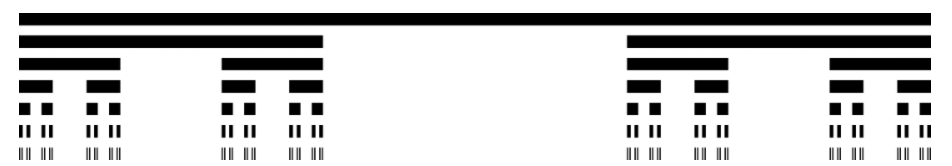
\includegraphics[width=0.65\textwidth]{graphics/Chap05/CantorSet02.png}
}
\hspace{5pt}%
\subfloat[]{%
    \label{fig:CantorSetB}%
	\centering
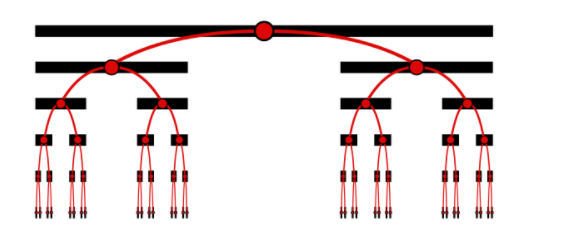
\includegraphics[width=0.3\textwidth]{graphics/Chap05/CantorSet.png}}%
\caption[]{Images of the Cantor set, thanks to Wikipedia. (a) The top line is the interval $[0, 1]$. The line below is what is left when one removes the (open) middle third, $(1/3, 2/3)$. The line below that is what is left when the next two (open) middle thirds, $(1/9, 2/9)$ and $(7/9, 8/9)$, are removed, etc. In the beginning, it's hard to believe that there is anything left over, but there is. In fact, the Cantor set can be placed in one to one correspondence with the original interval $[0,1]$. (b) Shows various paths traced out in a ternary (base 3) expansion of numbers in the Cantor set; ``each point in the Cantor set is uniquely located by a path through an infinitely deep binary tree, where the path turns left or right at each level according to which side of a deleted segment the point lies on. Representing each left turn with 0 and each right turn with 2 yields the ternary  [expansion] for a point'', from Wikipedia \url{https://en.wikipedia.org/wiki/Cantor_set}. Replacing the 2's with 1's  yields a bijection from the Cantor set to the interval $[0, 1]$, which is cool and surprising, though otherwise irrelevant to ROB 501! 
} 
    \label{fig:CantorSet}
\end{figure}

The Cantor set $C \subset [0, 1]$ is a famous set that is uncountable and has Lebesgue measure $0$, 
$$C= \left\{ x \in [0, 1] ~\left|~ x= \sum_{i=1}^\infty  \frac{\epsilon_i}{3^i}, \epsilon_i \in \{0, 2\} \right.  \right\}.$$
The classical construction given in \url{https://en.wikipedia.org/wiki/Cantor_set} shows that it belongs to the Borel sigma algebra. 
% Indeed, if one defines $C_0=[0,1]$, and $ C_{n}:={\frac {C_{n-1}}{3}}\cup \left({\frac {2}{3}}+{\frac {C_{n-1}}{3}}\right)={\frac {1}{3}}{\bigl (}C_{n-1}\cup \left(2+C_{n-1}\right){\bigr )}$, then 
% $$C:=}{\displaystyle {\color {Blue}\lim _{n\to \infty }C_{n}}}{\displaystyle {\color {Blue}\lim _{n\to \infty }C_{n}}}{\displaystyle =\bigcap _{n=0}^{\infty }C_{n}=\bigcap _{n=m}^{\infty }C_{n}}{\displaystyle =\bigcap _{n=0}^{\infty }C_{n}=\bigcap _{n=m}^{\infty }C_{n}}   for any   {\displaystyle m\geq 0}{\displaystyle m\geq 0.
It is impossible to define a uniform probability measure on $[0,1]$ and compute the probability of the Cantor set by performing a Riemann–Stieltjes integral over $C$ because the ``index function'' 
$$ I(x) =  \begin{cases}    1 &  x \in C \\ 0 & \text{ otherwise} \end{cases} $$
has unbounded variation \url{https://en.wikipedia.org/wiki/Bounded_variation}. Said another way, 
$$ P(C) := \underset{ C }{\int}  dx= \int_{0}^{1} I(x)~ dx = \text{ undefined as a Riemann or Riemann–Stieltjes integral}.$$

In any case, whether you are convinced or not, in the rest of this Chapter, we are obliged to be less careful than we have been in other parts of the book. When we discuss the probability of an event and compute it via an integral, we will simply assume that the integral exists within the usual theory of Riemann integration.

\section{First Pass on Probability Basics}
We assume that you may have skipped directly to here.

\subsection{Densities and Random Variables}

\begin{definition}
\label{def:ProbSpaceCopy2}
 $(\Omega, \mathscr{F}, P)$ is called a \textbf{probability space}.
\begin{itemize}
\item $\Omega$ is the sample space. Think of it as the set of all possible outcomes of an experiment. 
\item $E \subset \Omega$ is an event.
\item $\mathscr{F}$ is the collection of allowed events\footnote{Though it is too deep for ROB 501, there are subsets of the reals, for example, that are so complicated one cannot define a reasonable notion of probability that agrees with how we would want to define the probability of an interval, such as $[a, b]$.}. It must at least contain $\emptyset$ and $\Omega$. It is closed with respect to set complement, countable unions, and countable intersections\footnote{By De Morgan's laws, once a set is closed under set complements and countable unions, it is automatically closed under countable intersections; see \url{https://en.wikipedia.org/wiki/De_Morgan}.}. Such sets are called sigma algebras \url{https://en.wikipedia.org/wiki/%CE%A3-algebra}.
    \item $P:\mathscr{F} \to [0, 1]$ is a probability measure. It has to satisfy a few basic operations
    \begin{enumerate}
    \item $P(\emptyset)=0$ and $P(\Omega)=1$.
    \item For each $E\in \mathscr{F}$, $0 \le P(E) \le 1$
    \item If the sets $E_1, E_2, \ldots $ are disjoint (i.e., $E_i \cap E_j = \emptyset$ for $i \neq j$), then
    $$P\big(\bigcup_{i=1}^{\infty}E_i\big) = \sum_{i=1}^{\infty} P(E_i). $$
    \end{enumerate}
    These are typically called the \textbf{Axioms of Probability}.
\end{itemize}
\end{definition}

Shortly, we will define a \emph{probability density}. On the one hand, a density can be viewed as allowing us to define a probability space on the range $\real$ of a random variable $X:\Omega \to \real$. On the other hand, it can be viewed as replacing all of the confusing probability space details with integrals over sets. It is fine to use the latter interpretation.

\begin{figure*}[bth]
	\centering
	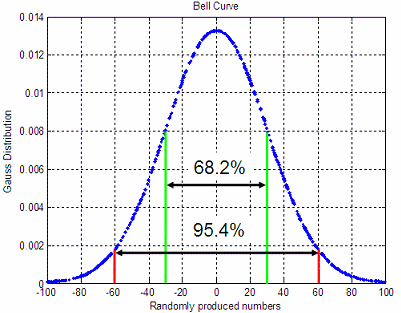
\includegraphics[width=0.35\columnwidth]{graphics/Chap05/gauss-distribution-002.png}~~~~~~ ~~~~
	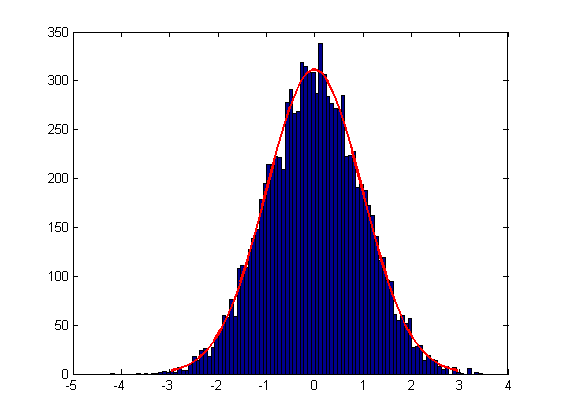
\includegraphics[width=0.35\columnwidth]{graphics/Chap05/O3lCB.png}
	\caption{(Left) Normal distribution $N(\mu, \sigma)$ with $\mu=0$ and $\sigma=30$. (Right) How do you determine the density? You have to collect data! The figure shows a ``fit'' of a normal distribution to data.}
\end{figure*}



\begin{definition} For $E\subset \Omega$, its \textbf{set complement} in $\Omega$ is often denoted in two ways,
$\sim E := E^c := \{ x \in \Omega~~ | ~ x \not \in E\}.$  Similarly, for $A \subset \real$, $\sim A := A^c := \{ x \in \real~ | ~ x \not \in A\}.$
\end{definition}

\begin{definition} A function $X: \Omega \to R$ is a \textbf{random variable} if $\forall ~x \in \real$, the set $\{\omega \in \Omega~| X(\omega) \le x\} \in \mathscr{F} $, that is $P(\{\omega \in \Omega~| X(\omega) \le x\})$ is defined. 
\end{definition}

\emph{With a random variable, we are typically interested in computing the probability that it takes values in a given set $A\subset \real$, that is, we seek to determine $P\{\omega \in \Omega~| X(\omega) \in A\}$.} With the ``frequentist'' interpretation, we are asking how ``frequently'' does $X$ take values in the set $A$. This seems quite difficult to compute because we need to compute first, the inverse image of the set $A$ under the function $X:\Omega \to \real$, 
\begin{equation}
    \label{eq:invImageA}
    \{\omega \in \Omega~| X(\omega) \in A\},
\end{equation}
and then secondly, compute the probability of this set using our probability space $(\Omega, \mathscr{F}, P)$. \emph{The notion of a \emph{density} allows us to circumvent the computation of \eqref{eq:invImageA} and work directly with the set $A$ itself.} \\


% \begin{definition} A (piecewise continuous\footnote{See \url{https://en.wikipedia.org/wiki/Piecewise} A square wave is a piecewise continuous function on $\real$ because one can decompose $\real$ into a countable disjoint union of half-open intervals on which the function is continuous}) function $f:\Omega \to [0, \infty)$ is a \emph{probability density} corresponding to $P$ if $\forall A \in \mathscr{F}$, $P(A) = \underset{ A }{\int} f(x)  dx := \int_{-\infty}^{\infty} I_A(x) f(x) dx$, where $I_A$ is the indicator function. We'll say that $(\Omega, \mathscr{F}, P, f)$ is a probability space with density $f$.
% \end{definition} 

\begin{definition} A (piecewise continuous\footnote{See \url{https://en.wikipedia.org/wiki/Piecewise} A square wave is a piecewise continuous function on $\real$ because one can decompose $\real$ into a countable disjoint union of half-open intervals on which the function is continuous}) function $f:\real \to [0, \infty)$ is a \textbf{probability density} if $\int_{-\infty}^\infty f(x) dx = 1.0$
\end{definition}

\begin{example} Some common densities include
\begin{itemize}
    \item \textbf{Uniform density}: for $a < b$,  $$f(x) = \begin{cases} \frac{1}{b -a} & x \in [a, b] \\ 0 & \text{otherwise}. \end{cases}$$
    \item \textbf{Laplace density}: for $b>0$, $\mu \in \real$, and $x \in (-\infty, \infty)$,
    $$f(x) = \frac{1}{2b} e^{-|x - \mu|/b}.$$
    The parameter $\mu$
 is the mean value, defined below.
 \item \textbf{Gaussian or Normal density}:  for $\sigma>0$, $\mu \in \real$, and $x \in  (-\infty , \infty)$, 
 $$f(x) = \frac{1}{\sigma \sqrt{2 \pi}} e^{-\frac{1}{2} \left( \frac{x - \mu}{\sigma} \right)^2 }.$$ The parameter $\mu$ is the mean value and $\sigma$ is the standard deviation; see below.
 \end{itemize}

\end{example}


\begin{definition} A function $X: \Omega \to R$ is a \textbf{continuous random variable} with density $f:\real \to [0, \infty)$ if 
\begin{enumerate}
\setlength{\itemsep}{.2cm}
\renewcommand{\labelenumi}{(\alph{enumi})}
\item it is a random variable, and 
\item $\forall ~x \in \real$, 
$P(\{\omega \in \Omega~| X(\omega) \le x\})= \int_{-\infty}^x f(\bar{x}) d \bar{x}$.
\end{enumerate}
The lower bound of $-\infty$ is for convenience. It can be replaced with $\inf \{X(\Omega) \subset \real\}$.
\end{definition}

\begin{notation} The notation $X \sim f$ is read as $X$ is distributed with density $f$ or that $X$ is a random variable with density $f$.
\end{notation}


\begin{rem} Useful shorthand notation $\{ X \le x\}:=\{\omega \in \Omega~| X(\omega) \le x\}$ and more generally, for $A\subset \real$, we define $\{ X \in A\}:=\{\omega \in \Omega~| X(\omega) \in A\}$. 
$\hfill \square$  \end{rem} 

\begin{rem} Because $\mathscr{F}$ is closed under set complements, (countable) unions, and (countable) intersections, we can assign probabilities to
\begin{enumerate}
\setlength{\itemsep}{.2cm}
\renewcommand{\labelenumi}{(\alph{enumi})}
     \item $\{ X > x\}=\sim \{ X \le x\} = \{ X \le x\}^{c}$
     \item  $\{ x < X \le y\}= \{ X > x\} \cap  \{ X \le y\}$
\end{enumerate}
and compute them via 
\begin{enumerate}
\setlength{\itemsep}{.2cm}
\renewcommand{\labelenumi}{(\alph{enumi})}
     \item $P(\{ X > x\})= \int_{x}^{\infty} f(x) dx$ and 
     \item  $P(\{ x < X \le y\})=\int_{x}^{y} f(x) dx$, as long as $x \le y$.
\end{enumerate}
These integrals are well defined when $f$ is piecewise continuous.
$\hfill \square$  \end{rem} 


\begin{rem}
For how general of a set $A\subset \real$ can we compute $P(\{ X \in A \})$? To understand this, we note that
\begin{equation}
\label{eq:IntegralOverA}
    P(\{ X \in A \}) :=  \int_{A} f(x) dx := \int_{-\infty}^{\infty} I_A(x) f(x) dx.
\end{equation} 
Because we are limiting ourselves to Riemann-Stiljes integrals, we need $I_A$ to be sufficiently ``nice'' that the product $I_A(x) f(x)$ has bounded variation. A sufficient condition is that $A$
can be expressed as a countable disjoint union of half-open intervals. This seems to be general enough for use in engineering.
$\hfill \square$  \end{rem}


\begin{definition} Moments
 \begin{itemize}
     \item Mean: $\mu:=\E \{ X\}:= \int_{-\infty}^{\infty} x f(x) dx$

     \item Variance: $\sigma^2:=\E \{ (X-\mu)^2)\}:= \int_{-\infty}^{\infty} (x-\mu)^2f(x) dx$ (Var. for short)

     \item Standard Deviation: $\sigma :=\sqrt{\sigma^2}$ (Std. Dev. for short)
     \end{itemize}

\end{definition}
 
% \begin{example}
% \textcolor{red}{\bf Add example for computing stuff.}
% \end{example}

    \subsection{Random Vectors and Densities}
   

\begin{definition}
 Let $(\Omega, \mathscr{F}, P)$ be a probability space. A function $X: \Omega \rightarrow \real^p$ is called a \textbf{random vector} if each component of $X=\left[ \begin{array}{ccc}
        X_1\\X_2\\\vdots\\X_p\end{array} \right]$ is a random variable, that is, $\forall~ 1 \le i \le p$, $X_i: \Omega \rightarrow \real$   is a random variable. 
\end{definition} 

Consequently, $\forall x \in \real^p $, the set $\{\omega \in \Omega \mid X(\omega) \le x\} \in \mathscr{F}$ (i.e., it is an allowed event), where the inequality is understood \textbf{pointwise}, that is,
        $$\{\omega \in \Omega \mid X(\omega) \le x \}:= \left\{\omega \in \Omega ~|~ \begin{bmatrix}X_1(\omega) \\X_2(\omega) \\ \vdots \\ X_p(\omega) \end{bmatrix} \le \begin{bmatrix} x_1 \\x_2 \\ \vdots \\ x_p \end{bmatrix}  \right\} :=\left\{\omega \in \Omega ~~|~~ \begin{bmatrix}X_1(\omega) \le x_1 \\X_2(\omega) \le x_2\\ \vdots \\ X_p(\omega) \le x_p\end{bmatrix} \right\} = \bigcap\limits^p_{i=1} \{\omega \in \Omega \mid X_i(\omega) \le x_i\}.$$

\begin{definition} $X: \Omega \rightarrow \real^p$ is a \textbf{continuous random vector} if there exists a \textbf{density} $f_X:\real^p \to [0, \infty)$ such that,
 $$\forall~x\in \real^P,~~P\big(\{ X \le x\} \big)= \int_{-\infty}^{x_p} ... \int_{-\infty}^{x_2} \int_{-\infty}^{x_1}f_X(\bar{x}_1,\bar{x}_2...\bar{x}_p) d \bar{x}_1 d \bar{x}_2 ... d \bar{x}_p.$$
 More generally, for all $A\subset \real^p$ such that the indicator function $I_A$ has bounded variation,
 $$ P\big(\{ X \in A\} \big)= \int_{-\infty}^{\infty} ... \int_{-\infty}^{\infty} \int_{-\infty}^{\infty} I_A(\bar{x}_1,\bar{x}_2...\bar{x}_p) f_X(\bar{x}_1,\bar{x}_2...\bar{x}_p) d \bar{x}_1 d \bar{x}_2 ... d \bar{x}_p.$$
\end{definition} 

\begin{notation} The notation $X \sim f$ is read as $X$ is distributed with density $f$ or that $X$ is a random vector with density $f$.
\end{notation}



\begin{definition} (Moments) Suppose $g: \real^p \to \real^k$
        $$\E\{g(X)\}:=\int_{\real^p}g(x)f_X(x)dx:=\int_{-\infty}^{\infty}...\int_{-\infty}^{\infty}g(x_1,...,x_p)f_X(x_1,...,x_p)dx_1...dx_p$$
\begin{itemize}
    \item  \textbf{Mean or Expected Value}$$\mu=\E\{X\}=\E\{\left[ \begin{array}{ccc}X_1\\\vdots\\X_p\end{array} \right]\}=\left[ \begin{array}{ccc}\E\{X_1\}\\\vdots\\ \E\{X_p\}\end{array} \right]=
        \left[ \begin{array}{ccc}\mu_1\\\vdots\\\mu_p \end{array} \right]$$
\item 
        \textbf{Covariance Matrices}$$\Sigma:={\rm cov}(X)={\rm cov}(X,X)=\E\{(X-\mu)(X-\mu)^T\}$$
        where $(X-\mu) \mbox{ is }p\times 1 \mbox{, } (X-\mu)^T \mbox{ is }1\times p\mbox{, } (X-\mu)(X-\mu)^T \mbox{ is }p\times p$
        
        \item \textbf{Variance:} ${\rm Var}(X):= \tr \Sigma := \sum_{i=1}^{p} \Sigma_{ii}$, where $\Sigma$ is the covariance of $X$.

\end{itemize}

\end{definition}
       
\begin{exercise}
  $\Sigma:={\rm cov}(X)={\rm cov}(X,X)$ is a positive semi-definite matrix.
\end{exercise}

\textbf{Solution:} For $ v \in \real^p$, we need to show that $v^\top \Sigma v\ge 0$, where $\Sigma := \E \{(X-\mu) \cdot (X-\mu)^\top \}$. 
\begin{align*}
    v^\top \Sigma v:=& v^\top \E \{(X-\mu) \cdot (X-\mu)^\top \} v \\ 
    =&  \E \{v^\top(X-\mu) \cdot (X-\mu)^\top v\}  \\
    =& \E \{ \left((X-\mu)^\top v\right)^\top \cdot \left((X-\mu)^\top v \right)\} \\
    =& \E\{|| (X-\mu)^\top v ||^2  \} \\
    =& \int_{\real^p} || (X-\mu)^\top v ||^2 f_X(x) dx \\
    \ge& ~ 0
\end{align*}
because the integral of a non-negative function over $\real^p$ is non-negative.
\Qed

\begin{definition} If $\Sigma >0$, then $\Sigma^{-1}$ is called the \textbf{information matrix}. The interpretation is that ``high variance'' means ``low information'' and vice versa.
\end{definition}

  
        
\section{Estimators}

\subsection{Best Linear Unbiased Estimator (BLUE)}

\textbf{Model:} The measurement is $y=Cx+\varepsilon$, $y\in \mathbb{R}^m$, $x \in \mathbb{R}^n$, $\E\{\varepsilon\}=0$, $\cov\{\varepsilon,\varepsilon\}=\E\{\varepsilon \varepsilon^\top \}=Q>0$, and
the columns of $C$ are linearly independent. \emph{We assume no stochastic (random) model for the unknown $x$.} In other words, $x\in \real^n$ is an unknown deterministic vector. It is emphasized that $\varepsilon$ and hence $y$ are random vectors while $x$ is not a random vector. Do not let the lowercase symbols being used for $y$, $\epsilon$, and $x$ distract you.\\

    \textbf{Seek:} An estimate $\widehat{x}$ of $x$ that satisfies:
    \begin{enumerate}
        \item \ul{Linear:} $\widehat{x}=Ky$ for some $n \times m$ matrix $K$.
        \item \ul{Unbiased for all $x\in \real^n$:} $\E\{ \widehat{x} - x \} =0 $ holds for all $x\in \real^n$. It needs to hold for all $x$ because $x$ can be an arbitrary value in $\real^n$.
        \item \ul{Best:} $\widehat{x}$ minimizes  $\E\{(\widehat{x} - x)^\top (\widehat{x} -x)\}=\E\{ \sum \limits_{i=1}^n |\widehat{x_i}-x_i|^2\} $, the variance of $\widehat{x} - x$.
    \end{enumerate}
    
\begin{claim} A linear estimate $\widehat{x}=Ky$ is unbiased if, and only if $KC=I$.
\end{claim}
\textbf{Proof:} 
\begin{align*}
    0 & = \E\{ \widehat{x} - x\} ~\forall x \in \real^n\\
    & \Updownarrow \\
     0 & = \E\{ Ky - x\}  ~\forall x \in \real^n\\
    & \Updownarrow \\
     0 & = \E\{ K(Cx+\varepsilon) - x\}  ~\forall x \in \real^n\\
    & \Updownarrow \\
        0 & = \E\{ (K C - I)x\} - \E\{K \varepsilon \}  ~\forall x \in \real^n \\
    & \Updownarrow \\
            0 & = (K C - I)x  ~\forall x \in \real^n\\
\end{align*}
where we used $\E\{\varepsilon\}=0$ by assumption and $ \E\{ (K C - I)x\}=(K C - I)x$ because $x$ is deterministic. Finally, $0=(K C - I)x  ~\forall x \in \real^n \iff KC-I =0_{n \times n}$ as can be seen by taking $x = e^i$, for $1 \le i \le n$.

$\hfill \square$


    \textbf{Aside:}~ For $v, w \in \real^n$, $ (v+w)^\top (v+w)=v^\top v+w^\top w+v^\top w+w^\top v =
        v^\top v+w^\top w+2v^\top w$ because $v^\top w $ is a scalar.\\
        
        Therefore, for an unbiased linear estimator,

    \begin{align*}
\E\{(\widehat{x} - x)^\top (\widehat{x} -x)\}& =\E\{(KCx-x+K\varepsilon)^\top (KCx-x+K\varepsilon)\}\\
        & =\E\{x^\top(KC - I)^\top(KC-I)x+2(K\varepsilon)^\top(KC-I)x+\varepsilon^\top  K^\top  K \varepsilon\} \\
         & =\E\{2(K\varepsilon)^\top(KC-I)x+\varepsilon^\top  K^\top  K \varepsilon\}\\
         &= \E\{ \varepsilon^\top  K^\top  K \varepsilon\}
    \end{align*}
Moreover, by using the properties of the trace, we have
    \begin{equation*}
        \varepsilon^\top K^\top K\varepsilon= \tr\left( \varepsilon^\top K^\top K\varepsilon \right)=\tr\left(K\varepsilon\varepsilon^\top K^\top\right).
    \end{equation*}
    and therefore,
    \begin{align*}
\E\{(\widehat{x} - x)^\top (\widehat{x} -x)\}&=\tr\E\{K\varepsilon\varepsilon^\top K^\top\}\\
        &=\tr(KQK^\top ).
    \end{align*}
Hence, 
$$ 
  \widehat{K}=\argmin_{KC = I}  \E\{(\widehat{x} - x)^\top (\widehat{x} -x)\} \iff     \widehat{K}=\argmin_{KC = I}  \tr(KQK^\top) 
$$

    \textbf{A simplifying observation:} If we partition $K$ into rows via 
    $$K= \begin{bmatrix}
        k_1\\
        k_2\\
        \vdots\\
        k_n
    \end{bmatrix}$$
then $K^\top =\begin{bmatrix}
        k_1^\top &   \dotsb &  k_n^\top
    \end{bmatrix}$
    and $ \tr\left(\begin{bmatrix}
            {k_1}\\
            \vdots\\
            {k_n}
            \end{bmatrix}Q\begin{bmatrix}k_1^\top & \dotsb& k_n^\top\end{bmatrix}\right) =\sum^{n}_{i=1}k_iQk_i^\top$. Moreover, 
    \begin{align*}
        KC= I_{n\times n} &\iff C^\top K^\top =I_{n\times n}\\
        &\iff C^\top \begin{bmatrix}k_1^\top &  \dotsb & k_n^\top\end{bmatrix}=\begin{bmatrix}e_1 & \dotsb & e_n\end{bmatrix}\\
        &\iff C^\top k_i^\top=e_i\ \ \ \ 1\leq i\leq n.
    \end{align*}
Hence, we have $n$-separate optimization problems involving the column vectors $k_i^\top $, namely
    \begin{equation*}
        \widehat{k}_i^\top = \argmin_{C^\top k_i^\top=e_i} k_i Q k_i^\top, ~1 \le i \le n.
    \end{equation*}
    From Proposition~\ref{prop:UnderDetermined} for underdetermined equations, we have
$$\widehat{k}_i^\top = Q^{-1}C(C^\top Q^{-1}C)^{-1}e_i,$$
which yields
$$ \widehat{K}^\top = \begin{bmatrix} \widehat{k}_1^\top & \cdots & \widehat{k}_n^\top \end{bmatrix}=Q^{-1}C(C^\top Q^{-1}C)^{-1}.$$
    \newline
    Therefore,
    \begin{equation*}
      \widehat{K}= (C^\top Q^{-1}C)^{-1}C^\top Q^{-1}.
      \end{equation*}
\vspace*{.2cm}

\begin{thm} \textbf{(BLUE)}
     Let $x\in\real^n$, $y\in\real^m$, $y=Cx+\varepsilon$, $\E\{\varepsilon\}=0$, $\E\{\varepsilon\varepsilon^\top\}=:Q>0$, and $\rank(C)=n$. The Best Linear Unbiased Estimator (BLUE) is $\widehat{x}=\widehat{K}y$ where
    \begin{equation*}
        \widehat{K}=\left(C^\top Q^{-1}C\right)^{-1}C^\top Q^{-1}.
    \end{equation*}
    Moreover, the covariance of the error is
    \begin{equation*}
        \E\{\left(\widehat{x}-x\right)\left(\widehat{x}-x\right)^\top\}=\left(C^\top Q^{-1}C\right)^{-1}.
    \end{equation*}

\end{thm}

\textbf{Proof:} The only thing left to show is the error covariance. From previous calculations,
    \begin{align*}
        \widehat{x}-x&=Ky-x\\
        &=KCx+K\varepsilon-x\\
        &=K\varepsilon~(\text{because}~KC=I)\\
        \therefore \E\{(\widehat{x}-x)(\widehat{x}-x)^\top\}&=\E\{(K\varepsilon)(K\varepsilon)^\top\}\\
        &=\E\{K\varepsilon\varepsilon^\top K^\top\}\\
        &=KQK^\top
    \end{align*}
    Hence, 
    \begin{align*}
        \E\{\left(\widehat{x}-x\right)\left(\widehat{x}-x\right)^\top\}&=KQK^\top\\
        &=\left(C^\top Q^{-1}C\right)^{-1}C^\top Q^{-1}QQ^{-1}C\left(C^\top Q^{-1}C\right)^{-1}\\
        &=\left(C^\top Q^{-1}C\right)^{-1}\left[C^\top Q^{-1}C\right]\left(C^\top Q^{-1}C\right)^{-1}\\
        &=\left(C^\top Q^{-1}C\right)^{-1}.
    \end{align*}
    
    \Qed
    
\begin{rem} \emph{Comparing Weighted Least Squares to BLUE:}
\begin{itemize}
    \item They are \ul{identical} when the weighting matrix is taken as the \ul{inverse} of the covariance matrix of the noise term: $W=Q^{-1}$. The inverse of the covariance matrix is called the \textit{information} matrix. Hence, there is low information when the variance (or covariance) is large.

        \item Another way to say this, if you solve a least squares problem with weight matrix $W>0$, you are implicitly assuming that your uncertainty in the measurements has zero mean and a covariance matrix of $Q=W^{-1}$.

            \item If you know the uncertainty has zero mean and a covariance matrix of $Q$, using $W=Q^{-1}$ makes a lot of sense. For simplicity, assume that $Q$ is diagonal. A large entry in $Q$ means high variance, which means the measurement is highly uncertain. Hence, the corresponding component of $y$ should not be weighted very much in the optimization problem....and indeed, taking $W=Q^{-1}$ does just that because, the weight term $W$ is small for large terms in $Q$.
            
            \item Weighted least squares was based on overdetermined systems of linear equations. To derive BLUE, we needed to understand  underdetermined systems of linear equations. That's kind of cool!
    \end{itemize}
       
$\hfill \square$  \end{rem}
    
 \subsection{Minimum Variance Estimator (MVE)}   
 
 \textbf{Model:} $y=Cx+\varepsilon, y\in \mathbb{R}^m, x \in \mathbb{R}^n, \text{and}~ \varepsilon\in \mathbb{R}^m,$ with the following stochastic assumptions:
 \begin{itemize}
     \item Zero Means: $E\{x\}=0, E\{\varepsilon\}= 0$. 
     \item Covariances: $E\{\varepsilon \varepsilon^\top \}=Q, E\{xx^\top \}= P, E\{\varepsilon x^\top \}=0$.
 \end{itemize}

\begin{rem}
       $E\{\varepsilon x^\top \}=0$ means that the state variables and noise terms are uncorrelated. Recall that uncorrelated does NOT imply independence, except for Gaussian random vectors.
$\hfill \square$  \end{rem} 

\textbf{Assumption:}  $Q\ge 0$, $P \ge 0$, and $CPC^\top +Q >0$.  (Will see why later.) We note that $Q>0 \implies CPC^\top +Q >0$ for all $m \times n$ matrices $C$. If $Q>0$, we do not need to assume the columns of $C$ are linearly independent. In fact, $C = 0_{m \times n}$ is possible.\\

\textbf{Objective:} We seek $\widehat{x}$ that minimizes the variance
$$E\{(\widehat x -x)^\top (\widehat x -x)\} = E\{ \sum\limits_{i=1}^n (\widehat x_i-x_i)^2\} = \sum\limits_{i=1}^n E\{ (\widehat x_i-x_i)^2 \}.$$

\begin{rem} As for BLUE, we see that there are $n$ separate optimization problems.
       We also see that a linear estimate $\widehat x = Ky$ would be automatically unbiased, because
$$ E\{\widehat x - x\}=E\{ Ky - x\} = E\{ KCx+K\varepsilon - x\} = (KC-I) E\{x\}+KE\{\varepsilon\}  = 0,$$
without imposing that $KC = I$. 
$\hfill \square$  \end{rem}


\textbf{Problem Formulation (the Unexpected Inner Product):} We will pose this as a minimum norm problem in an inner product space of random variables. Suppose that 
$$x=   \begin{bmatrix}
    x_1\\
    \vdots\\
    x_n
  \end{bmatrix}~~~\text{and} ~~~~\varepsilon =   \begin{bmatrix}
    \varepsilon_1\\
    \vdots\\
    \varepsilon_m
  \end{bmatrix}.$$
  We recall that components of random vectors are random variables. Hence, $x_i$, $1 \le i \le n$ and $\varepsilon_j$, $1 \le j \le m$ are all random variables, and hence are \textbf{functions}.
  We define ${\cal F} = \mathbb{R},$ and $\mathcal{X} = span\{x_1, x_2, \dots , x_n, \varepsilon_1, \varepsilon_2, \dots, \varepsilon_m\},$ and for  $z_1,z_2 \in \mathcal{X}$, we \underline{define their inner product} by  $$<z_1,z_2> := E\{z_1z_2\}.$$
  We note that $\forall~ z \in \mathcal{X}$, $\E\{z\}=0$ and $\var(z)=<z,z>$. \textbf{Hence, this inner product space is designed to treat minimum variance optimization problems.}
  
  \begin{rem}
  $$ E\{z_1z_2\} = \begin{cases} P_{ij} & z_1 = x_i, z_2 = x_j \\  Q_{ij} & z_1 = \varepsilon_i, z_2=\varepsilon_j \\ 0 &  z_1 = x_i, z_2=\varepsilon_j \\ 0 &  z_1 = \varepsilon_i, z_2=x_j. \end{cases}$$
  $\hfill \square$  \end{rem}

\textbf{Define:} \\
$M = \spanof{y_1,y_2,\dots,y_m} \subset \mathcal{X}$ ($M$ is the subspace spanned by the measurements),\\

$y_i = C_ix+\varepsilon_i = \sum\limits_{j=1}^n C_{ij}x_j+\varepsilon_i, 1\le i \le m,$  ($i$-th row of $y$)\\

$\widehat{x}_i = \argmin\limits_{m \in M} \|x_i-m\|^2 =  \argmin \limits_{m \in M}  \langle x_i-m, x_i-m \rangle $\\


\textbf{Fact:} $\{y_1,y_2,\dots,y_m\}$ is linearly independent if, and only if, $CPC^\top +Q$ is positive definite. This is proven below when we compute the Gram matrix. (Recall, $\{y_1,y_2,\dots,y_m\}$ linearly independent if, and only if $G$ is full rank, where $G_{ij}:=<y_i,y_j>.$)\\


\textbf{ Solution via the Normal Equations:} By the normal equations,
$$\widehat{x}_i = \widehat \alpha_1 y_1  +  \widehat \alpha_2 y_2  + \dots + \widehat \alpha_m y_m$$
where $G^\top \widehat \alpha = \beta$ and
\begin{align*}
G_{ij} = <y_i,y_j> = E\{y_i y_j\} &= E\{[C_i x+\varepsilon_i][C_j x+\varepsilon_j]\}\\
& = E\{[C_i x+\varepsilon_i][C_j x+\varepsilon_j]^\top \}\\
& = E\{[C_i x+\varepsilon_i][x^\top  {C_j}^\top  +\varepsilon_j]\}\\
& = E\{C_i xx^\top  C_j^\top \} + E\{C_i x\varepsilon_j\} + E\{\varepsilon_i x^\top  C_j^\top \} + E\{ \varepsilon_i \varepsilon_j\}\\
& = C_iE\{ xx^\top  \}C_j^\top  + E\{ \varepsilon_i \varepsilon_j\}\\
& = C_i P C_j^\top  + Q_{ij}\\
&=[CPC^\top +Q]_{ij}\
\end{align*}
where we have used the fact that $x$ and $\varepsilon$ are uncorrelated. We conclude that
$$G = CPC^\top +Q.$$

We now turn to computing $\beta$. Let's note that $x_i$, the $i$-th component of $x$, is equal to $x^\top  e_i$, where $e_i$ is the standard basis vector in $\real^n$.
\begin{align*}
\beta_j = <x_i,y_j> &= E\{x_i y_j\}\\
 &= E\{x_i[C_j x+\varepsilon_j]\} \\
 &= E\{x_i C_j x\} + E\{x_i \varepsilon_j\} \\
 & = C_jE\{ x x_i\} \\
  & = C_jE\{ x x^\top  e_i\} \\
    & = C_jE\{ x x^\top  \} e_i\\
 &= C_j P e_i \\
 &= C_j P_i
\end{align*}
where $P=\begin{bmatrix} P_1 & P_2 &  \cdots & P_n \end{bmatrix}$, and hence $P_i$ is the $i$-th column of $P$. Putting all of this together, we have
\begin{align*}
G^\top \widehat \alpha &= \beta \\
&\Updownarrow \\
[CPC^\top +Q] \widehat \alpha &= C P_i \\
&\Updownarrow \\
\widehat \alpha &= [CPC^\top +Q]^{-1} C P_i
\end{align*}


$\widehat{x}_i = \widehat \alpha_1 y_1  +  \widehat \alpha_2 y_2  + \dots + \widehat \alpha_m y_m = \widehat \alpha^\top  y=$ (row vector $\times$ column vector), where
$$\widehat \alpha =   \begin{bmatrix}
    \widehat \alpha_1\\
    \vdots\\
    \widehat \alpha_m
  \end{bmatrix}.$$

We now seek to identify a gain matrix $K$ so that
$$\widehat x = Ky \iff \widehat x_i = K_i y, \text{where}~~K =    \begin{bmatrix}
   {K_1}\\
{K_2}\\
    \vdots\\
  {K_n}
  \end{bmatrix};$$
  that is, $K_i$ is the $i$-th row of $K$.

  \begin{align*}
    K_i^\top  = \widehat \alpha_i &=  [CPC^\top +Q]^{-1} C P_i, 1 \le i \le n\\
    &\Updownarrow\\
   \begin{bmatrix} K_1^\top  & \cdots & K_n^\top  \end{bmatrix} &= [CPC^\top +Q]^{-1} C P\\
   &\Updownarrow\\
   K^\top &=  [CPC^\top +Q]^{-1} C P\\
   &\Updownarrow\\
    K&=PC^\top [CPC^\top +Q]^{-1}\
\end{align*}

$$\boxed{\widehat{x} = K y =  PC^\top [CPC^\top +Q]^{-1}y}$$

\begin{thm} \textbf{(Minimum Variance Estimator)}
\label{thm:MVE}
     Let $x\in\real^n$, $y\in\real^m$, $y=Cx+\varepsilon$,  with the following stochastic assumptions:
 \begin{itemize}
     \item Zero Means: $E\{x\}=0, E\{\varepsilon\}= 0$. 
     \item Covariances: $E\{\varepsilon \varepsilon^\top \}=Q, E\{xx^\top \}= P, E\{\varepsilon x^\top \}=0$.
 \end{itemize} 
The Minimum Variance Estimator (MVE) is $\widehat{x}=\widehat{K}y$ where
    \begin{equation*}
        \widehat{K}=PC^\top [CPC^\top +Q]^{-1}.
    \end{equation*}
    Moreover, the covariance of the error is
    \begin{equation*}
        \E\{\left(\widehat{x}-x\right)\left(\widehat{x}-x\right)^\top\}=P-PC^\top [CPC^\top +Q]^{-1}CP.
    \end{equation*}

\end{thm}

\textbf{Proof:} The only thing left to show is the error covariance. From previous calculations,  let's note that
$$\widehat x -x = Ky-x = KC x + K \varepsilon  - x=(KC - I)x + K \varepsilon $$
and thus
$$ (\widehat x -x)(\widehat x -x)^\top= (KC - I)x x^\top (KC - I)^\top + K \varepsilon \varepsilon^\top K^\top - (KC - I)x \varepsilon^\top K^\top - K\varepsilon x^\top (KC - I)^\top.  $$

Taking expectations, and recalling that $x$ and $\varepsilon$ are uncorrelated, we have
\begin{align*}
E\{(\widehat x -x)(\widehat x -x)^\top \} & = (KC-I) P (KC-I)^\top + K Q K^\top \\
&= KC P C^\top K^\top + P - 2 PC^\top K^\top + K Q K^\top\\
&= P + K [CPC^\top + Q] K^\top  -2 PC^\top K^\top.
\end{align*}
Substituting with $K=PC^\top [CPC^\top +Q]^{-1}$ and simplifying yields the result.
\Qed

\newpage

\begin{rem} \mbox{ }

\begin{enumerate}
\item $\cov(\begin{bmatrix} x \\ y \end{bmatrix}) = \E\{\ \left[\begin{array}{c} x \\ Cx + \varepsilon  \end{array} \right] \left[\begin{array}{cc} x^\top & x^\top C^\top + \varepsilon^\top \end{array} \right] \} = \left[\begin{array}{cc} P & P C^\top \\ C P & CPC^\top + Q \end{array} \right].$

\item Hence, we see that the covariance of the error $\widehat{x}-x$ is the Schur Complement of $\cov(x)$  in  $\cov(\begin{bmatrix} x \\ y \end{bmatrix})$. 

\item The term $PC^\top [CPC^\top +Q]^{-1}CP$ represents the ``value'' of the measurements. It is the reduction in the covariance of $x$ given the measurement $y$.

\item If $Q>0$ and $P>0$, then from the Matrix Inversion Lemma
$$\boxed{\widehat x = Ky = [C^\top Q^{-1}C+P^{-1}]^{-1}C^\top Q^{-1}y.}$$
This form of the equation is useful for comparing BLUE vs MVE

\item \textbf{BLUE vs MVE:}\\

\begin{itemize}

\item \textbf{BLUE:} $\widehat x = [C^\top  Q^{-1}C]^{-1}C^\top  Q^{-1}y$ \\

\item \textbf{MVE:} $\widehat x = [C^\top  Q^{-1}C+P^{-1}]^{-1}C^\top  Q^{-1}y$ \\

\item Hence, BLUE = MVE when $P^{-1} = 0$.\\

\item $P^{-1} = 0$ roughly means $P= \infty I$, that is infinite covariance in $x$, which in turn means we have \textit{no idea} about how $x$ is distributed.\\

    \item For BLUE to exist, we need $\dim(y) \ge \dim(x) $\\

    \item For MVE to exist, we can have $\dim(y) < \dim(x) $ as long as $(C P C^\top + Q) >0$.

\end{itemize}

\end{enumerate}

       
$\hfill \square$  \end{rem}

\begin{rem} (Solution to MIL) We will show that if $Q>0$ and $P>0$, then 
$$ PC^\top [CPC^\top +Q]^{-1}= [C^\top  Q^{-1}C+P^{-1}]^{-1}C^\top  Q^{-1}.$$

Recall the MIL: Suppose that $A$, $B$, $C$ and $D$ are compatible\footnote{The sizes are such the matrix products and sum in $A+BCD$ make sense.} matrices. If $A$, $C$, and  $(C^{-1}+D A^{-1}B)$ are each square and invertible, then  $A+BCD$ is invertible and
    $$ (A + BCD)^{-1} = A^{-1} - A^{-1}B(C^{-1} + DA^{-1}B)^{-1}DA^{-1}.$$

We apply the MIL to $[C^\top  Q^{-1}C+P^{-1}]^{-1}$, where we identify $A=P^{-1}, B=C^\top, C=Q^{-1}, D=C$. This yields
$$[C^\top  Q^{-1}C+P^{-1}]^{-1} = P-PC^\top [ Q + CPC^\top]^{-1} CP.$$
Hence,
\begin{align*}
[C^\top  Q^{-1}C+P^{-1}]^{-1}C^\top  Q^{-1} &= PC^\top  Q^{-1}-PC^\top [ Q + CPC^\top]^{-1} CPC^\top  Q^{-1} \\
&= PC^\top \left[ I - [Q+CPC^\top]^{-1} CPC^\top   \right] Q^{-1} \\
&={\scriptstyle  PC^\top \left[ [Q+CPC^\top]^{-1} [Q+CPC^\top] - [Q+CPC^\top]^{-1} CPC^\top   \right] Q^{-1}}\\
&=PC^\top [Q+CPC^\top]^{-1} \left[  [Q+CPC^\top] - CPC^\top   \right] Q^{-1}\\
&= PC^\top [Q+CPC^\top]^{-1} \left[  Q+CPC^\top - CPC^\top   \right] Q^{-1}\\
&= PC^\top [Q+CPC^\top]^{-1} \left[  Q    \right] Q^{-1}\\
&= PC^\top [Q+CPC^\top]^{-1}
\end{align*}

$\hfill \square$  
\end{rem}

\section{Second Pass on Probability Basics}
    
    
   \subsection{Marginal Densities, Independence, and Correlation}
        Suppose the random vector $X: \Omega \rightarrow \real^p$ is partitioned into two components $X_1 : \Omega \rightarrow R^n$ and $X_2:\Omega \rightarrow R^m $, with $p=n+m$, so that,
        $$ X = \left[ \begin{array}{cc} X_1 \\
                                               X_2 \end{array} \right]$$

\begin{notation} We denote the density of $X$ by

$$f_X(x)=f_{\small \left[ \begin{array}{cc} X_1 \\
                                               X_2 \end{array} \right]}(x_1,x_2)=f_{X_1 X_2}(x_1,x_2) $$

and it is called the \textbf{joint density} of $X_1$ and $X_2$. As before, we can define the mean and covariance.
\begin{itemize}

 \item Mean is $\mu=
        \left[ \begin{array}{ccc}\mu_1\\ \mu_2 \end{array} \right]= \E\{X\}=\E\{\left[ \begin{array}{ccc}X_1\\ X_2\end{array} \right]\}=\left[ \begin{array}{ccc}\E \{X_1\}\\ \E\{X_2\}\end{array} \right]$

 \item Covariance is \begin{align*} \Sigma =    \left[ \begin{array}{cc}\Sigma_{11} & \Sigma_{12}\\ \Sigma_{21} & \Sigma_{22}\end{array} \right] &= \E\{\left[ \begin{array}{c}X_1-\mu_1\\ X_2-\mu_2\end{array} \right] \left[ \begin{array}{c}X_1-\mu_1\\ X_2-\mu_2\end{array} \right]^\top\}  \\
     &= \E\{\left[ \begin{array}{c}X_1-\mu_1\\ X_2-\mu_2\end{array} \right] \left[ (X_1-\mu_1)^\top~~~ (X_2-\mu_2)^\top  \right] \} \\
     &= \E\{\left[ \begin{array}{cc}(X_1-\mu_1)(X_1-\mu_1)^\top &(X_1-\mu_1)(X_2-\mu_2)^\top \\
     (X_1-\mu_1)(X_2-\mu_2)^\top &(X_2-\mu_1)(X_2-\mu_2)^\top
     \end{array} \right]
     \end{align*}
 \end{itemize}
 where $\Sigma_{12}=\Sigma_{21}^\top = cov(X_1,X_2)=\E\{ (X_1-\mu_1)(X_2-\mu_2)^\top  \}$ is also called the \textbf{correlation} of $X_1$ and $X_2$.

\end{notation}

 If $X = \left[ \begin{array}{cc} X_1 \\
                                               X_2 \end{array} \right] :\Omega \to \real^{n+m}$ is a continuous random vector, then its components
                                               $$X_1:\Omega \to \real^n~~\text{and}~~X_2: \Omega \to \real^m$$ are also continuous random vectors and have densities, $f_{X_1}(x_1)$ and $f_{X_2}(x_2)$. These densities are given a special name. 

\begin{definition} $f_{X_1}(x_1)$ and $f_{X_2}(x_2)$  are called the \textbf{marginal densities} of $X_1$ and $X_2$.
       
\end{definition}

\begin{fact} In general the marginal densities are a nightmare to compute.  \begin{align*} f_{X_1}(x_1) &:= \int_{-\infty}^{\infty} f_{X_1 X_2}(x_1, x_2) d x_2  \medskip \\
 &: =\int_{-\infty}^{\infty} \cdots \int_{-\infty}^{\infty} f_{X_1X_2}\big( \underbrace{ \bar{x}_1, \ldots, \bar{x}_n }_{x_1}, \underbrace{ \bar{x}_{n+1} , \cdots, \bar{x}_{n+m}}_{x_2} \big) \underbrace{d\bar{x}_{n+1} \cdots d\bar{x}_{n+m}}_{dx_2}\\
 \\
 f_{X_2}(x_2) &:= \int_{-\infty}^{\infty} f_{X_1 X_2}(x_1, x_2) d x_1  \medskip \\
 &: =\int_{-\infty}^{\infty} \cdots \int_{-\infty}^{\infty} f_{X_1X_2}\big( \underbrace{ \bar{x}_1, \ldots, \bar{x}_n }_{x_1}, \underbrace{ \bar{x}_{n+1} , \cdots, \bar{x}_{n+m}}_{x_2} \big) \underbrace{d\bar{x}_{1} \cdots d\bar{x}_{n}}_{dx_1}\\
\end{align*}
For Normal Random Vectors, however, we can read the marginal densities directly from the joint density! We will not be doing any iterated integrals in ROB 501.
 
$\hfill \square$  \end{fact} 

\begin{definition} Random vectors $X_1$ and $X_2$ are \textbf{independent} if their joint density factors
        $$f_X(x)=f_{X_1 X_2}(x_1,x_2)=f_{X_1}(x_1)f_{X_2}(x_2).$$

$X_1$ and $X_2$ are \textbf{uncorrelated} if their ``cross covariance'' or ``correlation '' is zero, that is, 
        $$cov(X_1,X_2) := \E \{ (X_1-\mu_1)(X_2-\mu_2)^\top \} = 0_{n \times m}.$$
       
\end{definition}

\begin{fact} If random vectors $X_1$ and $X_2$ are independent, then they are also uncorrelated. \textcolor{red}{\bf The converse is in general false.}
$\hfill \square$
\end{fact} 

\subsection{Conditional Probabilities}

\begin{definition} Consider two events $A,B \in \mathscr{F}$, with $P(B) > 0$. The \textbf{conditional probability of $A$ given $B$} is
        $$P(A \mid B):=\frac{P(A\bigcap B)}{P(B)}.$$
\end{definition} 

\begin{rem} Suppose $A$ is the event that our robot is near a certain location and $B$ is the event that our robot has been cited by a particular camera. These two events have individual probabilities $P(A)$ and $P(B)$. The \textbf{conditional probability of event $A$ given that event $B$ occurred is how we ``fuse'' the two pieces of information},
        $$P(A \mid B):=\frac{P(A\bigcap B)}{P(B)}.$$
As an example, suppose we define a uniform probability across all floors of FRB, which has a total surface area of roughly 12,000 $m^2$ (roughly, 120,000 square feet) and let $A$ be the event our robot is choosing a snack in the self-service section of the Eigen Cafe. Well, the area of the self-service section of the Eigen Cafe is roughly 8 $m^2$, and thus $P(A) \approx 6.66~10^{-4}$. We'll now let $B$ be the event that our robot has been seen (i.e, measured to be) at the Eigen Cafe. The total area of the Eigen Cafe is approximately 30 $m^2$. Hence, $P(B)\approx 2.5~ 10^{-3}$. Because $A \subset B$, it follows that $A \cap B = A$ and hence
    $$P(A \mid B)=\frac{P(A\bigcap B)}{P(B)} = \frac{P(A)}{P(B)}= \frac{6.66~10^{-4}}{2.5~ 10^{-3}}=0.266.$$
    We note that $P(A \mid B)=0.266$ is a lot more certain than $P(A) \approx 6.66~10^{-4}$. Hence, as you can now imagine, conditional probabilities are very important in engineering.
$\hfill \square$  \end{rem}

\begin{rem} Special cases:
\begin{itemize}
        \item
        $B\subset A \mbox{, } P(A \mid B)=\frac{P(A\bigcap B)}{P(B)}=\frac{P(B)}{P(B)}=1$
        \item
        $A\subset B \mbox{, } P(A \mid B)=\frac{P(A\bigcap B)}{P(B)}=\frac{P(A)}{P(B)}\ge P(A)$

        \end{itemize}
        
$\hfill \square$  \end{rem}
   
   \begin{definition} Consider again our partitioned random vector 
   $ X = \left[ \begin{array}{cc} X_1 \\ X_2 \end{array} \right]$. The \textbf{conditional density of $X_1$ given $X_2 = x_2$} is
          $$f_{X_1\mid X_2}(x_1 \mid x_2):=\frac{f_{X_1X_2}(x_1,x_2)}{f_{X_2}(x_2)}.$$
        Sometimes, for brevity, we simply write $f(x_1 \mid x_2)$.
 \end{definition} 
 
 \begin{rem} \textbf{Remarks on Conditional Random Vectors:}
        \begin{itemize}

        \item \textbf{Very important:} $X_1$ given $X_2=x_2$ is (still) a random vector. It's density is $f_{X_1\mid X_2}(x_1 \mid x_2)$

        \item \textbf{Conditional Mean:} \begin{align*} \mu_{X_1 \mid X_2=x_2}&:=\E \{ X_1 \mid X_2=x_2\}  \\ &:=\int_{-\infty}^{\infty} x_1 f_{X_1\mid X_2}(x_1 \mid x_2) dx_1
            \end{align*}
            $\mu_{X_1 \mid X_2=x_2}$ is a function of $x_2$. Think of it as a function of the value read by your sensor.

         \item  \textbf{Conditional Covariance:} \begin{align*} \Sigma_{X_1 \mid X_2=x_2} & := \E \{ (X_1 -\mu_{X_1 \mid X_2=x_2})(X_1 -\mu_{X_1 \mid X_2=x_2})^\top \mid X_2=x_2 \} \\ \\ &:=\int_{-\infty}^{\infty} (X_1 -\mu_{X_1 \mid X_2=x_2})(X_1 -\mu_{X_1 \mid X_2=x_2})^\top f_{X_1\mid X_2}(x_1 \mid x_2) dx_1
            \end{align*}
            $\Sigma_{X_1 \mid X_2=x_2}$ is a function of $x_2$. Think of it as a function of the value read by your sensor.

        \end{itemize}



 
 $\hfill \square$  \end{rem}
       


       \subsection{(Optional Read) Derivation of the Conditional Density Formula from the Conditional Distribution:}
       
       \begin{definition} Let $X : \Omega \to \real^p$ be a random vector. Then $F: \real^p \to [0, 1]$ is a \textbf{cumulative probability distribution function} if $\forall~x\in \real^p$, $F(x) = P(\{ X \le x\})$.
       \end{definition}
       
       \begin{rem}
              If $X\sim f$, then the cumulative distribution function and the density are related by $F(x) = \int_{-\infty}^{x} f(x) dx$ and $f(x) = \frac{\partial}{\partial x} F(x)$. By the definition of a density, the integral is well defined. 
             $\hfill \square$  \end{rem}
       
      We define $A:=\{X_1 \le x_1 \}$ and for $\epsilon >0$, define $B_\epsilon:=\{x_2 - \epsilon \le X_2 \le x_2+\epsilon \}$ where $x_2\pm \epsilon$ means adding or subtracting $\epsilon$ to each component of $x_2$. Then,

\begin{align*}
P(A\bigcap B_{\epsilon})&=\int^{x_1}_{-\infty}\int^{x_2+\epsilon}_{x_2-\epsilon}f_{X_1X_2}(\bar{x}_1,\bar{x}_2)d\bar{x}_2d\bar{x}_1 \\
        P(B_{\epsilon})&=\int^{x_2+\epsilon}_{x_2-\epsilon}f_{X_2}(\bar{x}_2)d\bar{x}_2 
\end{align*}
Moreover, applying l'H\^{o}pital's Rule, 
\begin{align*}
        F_{X_1 \mid X_2}(x_1\mid x_2) &= \lim_{\epsilon \to 0}\frac{P(A\bigcap B_{\epsilon})}{P(B_{\epsilon})} \\
        &=\lim_{\epsilon \to 0}\frac{\int^{x_1}_{-\infty}\int^{x_2+\epsilon}_{x_2-\epsilon}f_{X_1X_2}(\bar{x}_1,\bar{x}_2)d\bar{x}_2d\bar{x}_1}
        {\int^{x_2+\epsilon}_{x_2-\epsilon}f_{X_2}(\bar{x}_2)d\bar{x}_2}\\
        &=\int^{x_1}_{-\infty}\lim_{\epsilon \to 0}\frac{\int^{x_2+\epsilon}_{x_2-\epsilon}f_{X_1X_2}(\bar{x}_1,\bar{x}_2)d\bar{x}_2}
        {\int^{x_2+\epsilon}_{x_2-\epsilon}f_{X_2}(\bar{x}_2)d\bar{x}_2} d\bar{x}_1\\
        &= \int^{x_1}_{-\infty} \frac{f_{X_1X_2}(\bar{x}_1,{x}_2)}{f_{X_2}({x}_2)} d\bar{x}_1.
\end{align*}
Differentiating the distribution function with respect to $x_1$ gives the density and hence
$$\left(  X_1\mid X_2=x_2 \right) \sim f_{X_1\mid X_2}(x_1 \mid x_2) = \frac{f_{X_1X_2}({x}_1,{x}_2)}{f_{X_2}({x}_2)}.$$

Alternatively, one can differentiate with respect to $x_1$ first, and then take the limit as $\epsilon \to 0$,
        $$f_{X_1 \mid X_2}(x_1\mid x_2)
        =\lim_{\epsilon \to 0} \frac{\int^{x_2+\epsilon}_{x_2-\epsilon}f_{X_1X_2}(x_1,\bar{x}_2)d\bar{x}_2}
        {\int^{x_2+\epsilon}_{x_2-\epsilon}f_{X_2}(\bar{x}_2)d\bar{x}_2}
        =\lim_{\epsilon \to 0} \frac{f_{X_1X_2}(x_1,x_2)\cdot 2\epsilon}{f_{X_2}(x_2)\cdot 2\epsilon}
        =\frac{f_{X_1X_2}(x_1,x_2)}{f_{X_2}(x_2)}.$$
        
        
\section{Important Facts about Gaussian Random Vectors}

\begin{definition} A \textbf{random variable} $X$ is \textbf{normally distributed} with mean $\mu$ and variance $\sigma^2 >0$ if it has density
$$ f_X(x) = \frac{1}{\sigma \sqrt{2 \pi}} e^{-\frac{(x-\mu)^2}{2 \sigma^2}}.$$

The standard deviation is $\sigma>0$. The mean and variance satisfy
\begin{align*} \mu &:= \E\{ X\} := \int_{\real} x f_X(x) dx := \int_{-\infty}^{\infty} x f_X(x) dx \\
\\
\sigma^2&:= \E\{ (X-\mu)^2 \} := \int_{\real} (x-\mu)^2 f_X(x) dx := \int_{-\infty}^{\infty} (x-\mu)^2 f_X(x) dx.
\end{align*}

\end{definition}

You should be quite familiar with the  ``bell curve''. $X$ is also called a Gaussian random variable.  We also say $X$ has a \textit{univariate normal distribution} or a \textit{univariate Gaussian distribution} to emphasize that we are talking about a single random variable.\\

For the most part, we do not care too much about individual random variables. We are interested in collections of random variables and random vectors, and hence we are primarily concerned about \textit{jointly distributed random variables}. If you take EECS 501, you can learn a tremendous amount of material about this subject. In the following, you will see a bare bones accounting of \textit{multivariate normal random variables}. 

\begin{definition} A finite collection of random variables $X_1, X_2, \cdots, X_p$, or equivalently, the random vector
 $$ X = \begin{bmatrix} X_1 \\ X_2 \\ \vdots \\ X_p  \end{bmatrix}$$
 has a (non-degenerate) \textbf{multivariate normal distribution} with mean $\mu$ and covariance $\Sigma>0$ if the joint density is given by
$$f_X(x) = \frac{1}{\sqrt{(2 \pi)^{p} |\Sigma| }} e^{ -\frac{1}{2} (x-\mu)^\top \Sigma^{-1}(x-\mu) }.$$

\end{definition}

In the above, $|\Sigma| = \det(\Sigma)$, which must be non-zero for the denominator to be well defined. This condition is what is meant by ``non-degenerate''. When $|\Sigma|=0$, one can still define a multivariate normal distribution, but the ``moment generating function'' must be used. This is a technicality that we will skip. We note that
\begin{align*}
\mu &:= \E\{ X\}  \in \real^p \\
\mu_i &:= \int_{\real^p} x_i ~f_X(x) dx := \int_{-\infty}^{\infty} \cdots \int_{-\infty}^{\infty}x_i ~ f_X(x_1,\cdots, x_p) dx_1 \cdots dx_p \\
\Sigma &:=\cov(X,X) :=\E\{ (X-\mu) (X-\mu)^\top \}  \in \real^{p \times p} \\
\Sigma_{ij} &:=\E\{ (X_i-\mu_i) (X_j-\mu_j)\} := \int_{\real^p} (x_i-\mu_i)(x_j - \mu_j) ~f_X(x) dx \\
x & = (x_1, x_2, \cdots, x_p) \text{ or } x= \begin{bmatrix} x_1 \\ x_2 \\ \vdots\\ x_p \end{bmatrix}~~\mbox{(depending on context)}.
\end{align*}


\begin{fact} \textbf{(Marginal Densities/Distributions)} Each random variable $X_i$ has a \textbf{univariate normal distribution} with mean $\mu_i$ and variance $\Sigma_{ii}$,
$$ f_{X_i}(x_i) = \frac{1}{ \sqrt{2 \pi \Sigma_{ii} }} e^{-\frac{(x_i-\mu_i)^2}{2 \Sigma_{ii}}}.$$
Hence, no iterated integrals are required to compute the marginal densities. Why is this true? Because the univariate density depends on two terms, namely, $\mu_i:=\E\{X_i\}$ and $\sigma_i^2:=\E\{(X_i-\mu_i)^2\}=\Sigma_{ii}.$
$\hfill \square$     \end{fact}


 We note the unfortunate lack of coordination in the notation: the standard deviation of $X_i$, which we typically denote by $\sigma_i$,  is given by
$$\sigma_i = \sqrt{\Sigma_{ii}}. $$
I guess we will not be denoting the entries of $\Sigma$ with lower case $\sigma$.


\begin{fact}\textbf{(Independence)}~Gaussian random variables are very special in that they are independent if, and only if, they are uncorrelated. Hence, $X_i$ and $X_j$ are \textit{independent} if, and only if, $\Sigma_{ij} = \Sigma_{ji}=0$.

$\hfill \square$  \end{fact}


\begin{fact}
\label{fact:GaussianLinearCombinations}
\textbf{(Linear Combinations)}~ Define a new random vector by $Y=A X + b$, with the rows of $A$ linearly independent. Then $Y$ is a Gaussian (normal) random vector with
\begin{align*}
   \E\{ Y\} &= A \mu + b=:\mu_Y\\
\cov(Y,Y)&=\E\{ (Y-\mu_Y) (Y-\mu_Y)^\top \} =A \Sigma A^\top =: \Sigma_{YY}.
\end{align*}
Indeed, $Y-\mu_Y = A(X-\mu)$. Hence,
$$\cov(Y,Y)=\E\{ [A(X-\mu)] [A(X-\mu)]^\top \} =A \E\{ (X-\mu) (X-\mu)^\top \}A^\top=A \Sigma A^\top,$$
and $A \Sigma A^\top >0$ when $A$ has full row rank and $\Sigma>0$.
$\hfill \square$  \end{fact}

\begin{rem}
       Taking $b=0$ and $A$ to be a row vector with all zeros except a one in the $i$-th spot, that is $A=[0, \cdots, 1, \cdots, 0]$, recovers the \textbf{marginal} densities discussed above.
$\hfill \square$  \end{rem} 

\section{Conditioning with Gaussian Random Vectors:}

\begin{rem} In various places,  $X_{|Y}$ and $X|Y$ are each used to represent $X$ conditioned on $Y=y$. 
\end{rem}

In addition to looking at individual random variables making up a random vector, we can group the components to form two or more blocks of vectors as long as their sizes add up to $p$, the number of components in $X$. We abuse notation and write
$$X = \begin{bmatrix} X_1 \\ X_2 \end{bmatrix} \begin{array}{c} \in \real^{n} \\ \in \real^{m} \end{array}$$
In books, you'll often see the blocks expressed in bold font, such as $\mathbf{X_1}$ and $\mathbf{X_2}$. We will NOT do this. Conformally with the partition of $X$ into two blocks, we partition the mean and covariance as follows
\begin{align*}
\mu &=: \begin{bmatrix} \mu_1 \\ \mu_2 \end{bmatrix}\\
 \Sigma &=: \left[ \begin{array}{cc} \Sigma_{11} & \Sigma_{12} \\ \Sigma_{21} & \Sigma_{22} \end{array}  \right].
\end{align*}
From our results on the Schur complement, we know that $\Sigma>0$ if, and only if, $\Sigma_{22}>0$ and $ \Sigma_{11}-\Sigma_{12} \Sigma_{22}^{-1}\Sigma_{21}>0$.

\begin{rem}
To be extra clear on the dimensions, we suppose $n+m=p$ and note that
\begin{align*}
\mu_1 &=  \E\{ X_1\} \in \real^n \\
\mu_2 &=  \E\{ X_2\} \in \real^m \\
\Sigma_{11} &= \cov(X_1,X_1)   \in \real^{n \times n}\\
\Sigma_{22} &=\cov(X_2,X_2)  \in \real^{m \times m}\\
\Sigma_{12} &= \cov(X_1,X_2)   \in \real^{n \times m} \\
\Sigma_{21} &=\cov(X_2,X_1) \in \real^{m \times n}.
\end{align*}
Furthermore, because $\Sigma=\Sigma^\top$, we have that
$$\Sigma_{11}^\top = \Sigma_{11},~~\Sigma_{22}^\top = \Sigma_{22},~\text{and } ~\Sigma_{12}^\top = \Sigma_{21}.$$
$\hfill \square$  \end{rem}

\begin{fact} Each vector  $X_i$ has a multivariate normal distribution with mean $\mu_i$ and covariance $\Sigma_{ii}$. This is also called the \textbf{marginal distribution} of $X_i$. If we know the mean and covariance for the composite vector $X$, it is very easy to read off the marginal distributions of its vector components. This can be established by Fact~\ref{fact:GaussianLinearCombinations} after writing $X_1= A_1 X + b_1$ with $b_1=0_{n \times 1}$ and $A_1 = [I_{n \times n}, 0_{n \times m}]$ and $X_2= A_2 X + b_2$ with $b_2=0_{m \times 1}$ and $A_2 = [0_{m \times n}, I_{m \times m}]$.
$\hfill \square$  \end{fact}




\begin{keyfact} 
\label{keyfact1}
 (Conditional Distributions of Gaussian Random Vectors:)~Let $X_1$ and $X_2$ be as above, namely they are components of a larger vector $X$ that has a multivariate normal distribution. Then the conditional distribution of $X_1$ given $X_2 = x_2$ has a multivariate normal distribution with
$$\text{Mean}:~~ \mu_{1|2}:= \mu_1 + \Sigma_{12} \Sigma_{22}^{-1} (x_2 - \mu_2)$$
and
$$\text{Covariance:}~~ \Sigma_{1|2}:= \Sigma_{11}-\Sigma_{12} \Sigma_{22}^{-1}\Sigma_{21}.$$
In passing, we note that the mean depends on the value of $x_2$ while the covariance does not.
$\hfill \square$
\end{keyfact}
To be extra clear on the meanings here, we note that
\begin{itemize}
\setlength{\itemsep}{.4cm}
\item $ \mu_{1|2} = \E\{ X_1~|~X_2 = x_2\}$
\item $ \Sigma_{1|2} = \E\{ (X_1-\mu_{1|2}) (X_1-\mu_{1|2})^\top~| ~X_2=x_2 \} $
\item $X_1$ given $X_2=x_2$ is a random vector. It has a multivariate normal distribution with the above mean vector and covariance matrix. Specifically, its density is
    $$f_{X_1|X_2=x_2}(x_1) = \frac{f_{X_1,X_2}(x_1,x_2) }{f_{X_2}(x_2)} = \frac{1}{\sqrt{(2 \pi)^{n} |\Sigma_{1|2}| } } e^{ -\frac{1}{2} (x_1-\mu_{1|2})^\top \Sigma_{1|2}^{-1}(x_1-\mu_{1|2}) }, $$
    where it is emphasized that $\mu_{1|2}$ depends explicitly on $x_2$.
\end{itemize}
 A proof of this can be found at the link below. The algebra is rather painful. If you are very ambitious, you can work out the special case where $X_1$ and $X_2$ are scalars. This will not be on any exam in ROB 501; see \url{http://fourier.eng.hmc.edu/e161/lectures/gaussianprocess/node7.html}; see also
 \url{http://www.stats.ox.ac.uk/~steffen/teaching/bs2HT9/gauss.pdf}.

\begin{rem} If $X_1$ and $X_2$ are uncorrelated, then $\mu_{1|2}=\mu_1$ and $\Sigma_{1|2} = \Sigma_{11}$. Similarly, let's suppose that $\Sigma_{22}$ is large, specifically, $\Sigma_{22}=\rho I_{m \times m}$. Then,
$\lim_{\rho \to \infty} \mu_{1|2}=\mu_1$ and $\lim_{\rho \to \infty} \Sigma_{1|2} = \Sigma_{11}$. The term $\Sigma_{12} \Sigma_{22}^{-1}\Sigma_{21}$ measures the value of the ``information gained by conditioning on  $X_2$''. As $ \Sigma_{22}^{-1} \to 0$, the value of the added information tends to zero.

$\hfill \square$  \end{rem}

\begin{keyfact} 
\label{keyfact2}
(Conditional Independence) Suppose we have 3 vectors $X_1$, $X_2$ and $X_3$ that are jointly normally distributed:
$$X = \begin{bmatrix} X_1 \\ X_2 \\ X_3 \end{bmatrix} $$
and that $X_1$ and $X_3$ are each independent of $X_2$. We then have no special structure on the means,
$$ \mu = \begin{bmatrix} \mu_1 \\ \mu_2 \\\mu_3\end{bmatrix} $$
but the covariance matrix has the form
$$ \Sigma = \left[ \begin{array}{ccc} \Sigma_{11} & 0 & \Sigma_{13} \\ 0 & \Sigma_{22} & 0 \\ \Sigma_{13}^\top & 0 & \Sigma_{33} \end{array}  \right]$$
where $\Sigma_{12}=\Sigma_{21}^\top=\cov(X_1,X_2)=0$ due to the independence of $X_1$ and $X_2$. Similarly for $\Sigma_{23}=\Sigma_{32}^\top=0$. Because $\Sigma$ is symmetric, $\Sigma_{31}=\Sigma_{13}^\top$.
\textbf{Then $X_1$ and $X_2$ are conditionally independent given $X_3$.} Written a different way, the two normal random variables, ${X_1}_{|X_3}$ ($X_1$ conditioned on knowing $X_3$) and  ${X_2}_{|X_3}$ ($X_2$ conditioned on knowing $X_3$) are independent.
 $\hfill \square$

\end{keyfact}

To see why this is true, we partition $\Sigma$ as
 $$ \Sigma = \left[ \begin{array}{cccc} \Sigma_{11} & 0 & |& \Sigma_{13} \\ 0 & \Sigma_{22} & | & 0 \\
 \cline{1-4}
  \Sigma_{13}^\top & 0 &| & \Sigma_{33} \end{array}  \right].$$
 We compute the covariance of $X_1$ and $X_2$ conditioned on $X_3$, that is
 $$ \left. \begin{bmatrix} X_1 \\ X_2  \end{bmatrix} \right| {X_3}, $$
using the Schur complement from \textbf{Key Fact~\ref{keyfact1}}
\begin{align*} \cov( \begin{bmatrix} {X_1}_{|X_3} \\ {X_2}_{|X_3}  \end{bmatrix} ,  \begin{bmatrix} {X_1}_{|X_3} \\ {X_2}_{|X_3}  \end{bmatrix}) &=  \left[ \begin{array}{cc} \Sigma_{11} & 0 \\ 0 & \Sigma_{22} \end{array}  \right] -  \left[ \begin{array}{c} \Sigma_{13} \\ 0 \end{array}  \right] \Sigma_{33}^{-1} \left[ \begin{array}{cc} \Sigma_{13}^\top & 0 \end{array}  \right]\\
&= \left[ \begin{array}{cc} \Sigma_{11} - \Sigma_{13}\Sigma_{33}^{-1} \Sigma_{13}^\top & 0 \\ 0 & \Sigma_{22} \end{array}  \right]
\end{align*}
Because the off-diagonal blocks are zero, the two random variables ${X_1}_{|X_3}$ and  ${X_2}_{|X_3}$ are uncorrelated, and because they are normal, we conclude they are independent.

\begin{mdframed} Once again, what we have seen is that if $X_1$ and $X_2$ are independent, and we also have $X_2$ is independent of $X_3$, then $X_1$ and $X_2$ remain independent when we condition them on $X_3$.
\end{mdframed} 


\begin{keyfact} 
\label{keyfact3}
(Covariance of a Sum of Independent Normal Random Variables) Let $X_1$ and $X_2$ be independent normal random vectors, with means $\mu_1$ and $\mu_2$, and covariances, $\Sigma_{11}$ and $\Sigma_{22}$. Define $Y$ as a ``linear combination'' of $X_1$ and $X_2$ via
 $$Y=A X_1 + BX_2$$
 for appropriately sized matrices $A$ and $B$. Then
 $$\mu_Y = A \mu_1 + B \mu_2$$
 and
 $$\cov(Y,Y) = A\Sigma_{11} A^\top + B \Sigma_{22} B^\top.$$
 $\hfill \square$
\end{keyfact} 

 To see why this is true, we first note that
\begin{align*}(Y-\mu_Y)(Y-\mu_Y)^\top &= A (X_1-\mu_1)(X_1-\mu_1)^\top A^\top +  B (X_2-\mu_2)(X_2-\mu_2)^\top B^\top \\
&~ +  A (X_1-\mu_1)(X_2-\mu_2)^\top B^\top + B (X_2-\mu_2) (X_1-\mu_1)^\top A^\top,
\end{align*}
and then note that when expectations are taken on each side, the independence of $X_1$ and $X_2$ gives
$${\cal E}\{ (X_1-\mu_1)(X_2-\mu_2)^\top \}=0 \text{ and } {\cal E}\{ (X_2-\mu_2)(X_2-\mu_2)^\top \}=0.$$
Therefore,
\begin{align*}
\cov(Y,Y) &= \E\{(Y-\mu_Y)(Y-\mu_Y)^\top  \}\\
&= A  {\cal E }\{ (X_1-\mu_1)(X_1-\mu_1)^\top \} A^\top +  B {\cal E}\{  (X_2-\mu_2)(X_2-\mu_2)^\top \} B^\top \\
&= A\Sigma_{11} A^\top + B \Sigma_{22} B^\top.
\end{align*}

\begin{keyfact} 
\label{keyfact4}
Suppose that $X$, $Y$ and $Z$ are jointly distributed random vectors with density $f_{X Y Z}$. Then the conditional random vectors $(X|Z)\big| (Y|Z)$ and $ X\big|\begin{bmatrix} Y \\ Z \end{bmatrix}$ have the same conditional densities, that is, 
$$ (X|Z)\big| (Y|Z) \sim \frac{f_{(X|Z)(Y|Z)}}{f_{(Y|Z)}}=\frac{f_{XYZ}}{f_{YZ}}\sim  X\big|\begin{bmatrix} Y \\ Z \end{bmatrix}.$$ 
$\hfill \square$

\end{keyfact}

The above fact does not require the random vectors to be jointly normal. The proof goes like this,
$$ (X|Z)\big| (Y|Z) \sim \frac{f_{(X|Z)(Y|Z)}}{f_{(Y|Z)}} = \frac{f_{\footnotesize{\left[\begin{array}{c}X\\ Y \end{array}\right] } \big| Z }}{f_{Y|Z}}=\frac{\frac{f_{XYZ}}{f_{Z}}}{\frac{f_{YZ}}{f_{Z}}}= \frac{f_{XYZ}}{f_{YZ}}\sim  X\big|\begin{bmatrix} Y \\ Z \end{bmatrix}.$$
In the Kalman Filter, the conditional density on the left will give us a recursive implementation of the density on the right, in place of a batch update. You have to see it in action to believe it.



 \section{Discrete-time Kalman Filter}  
    
 \subsection{Model and Assumptions}   
    
\textbf{Model:}~Linear time-varying discrete-time system with ``white\footnote{Recall that in white light, all frequencies are present. When only certain frequency components are present, you get ``colored'' light, such as blue light or red light. The term ``white'' noise means that if you compute the power spectral density of the noise random process, it is a constant, meaning that all frequency components are equally represented, just as in white light. }'' Gaussian noise
\begin{align*}
x_{k+1} &= A_k x_k + G_k w_k,~~x_0~\text{initial condition}\\
y_k &= C_k x_k + v_k
\end{align*}
$x\in \real^n$, $w \in \real^p$, $y\in \real^m$, $v\in \real^m$. Moreover, the random vectors
$x_0$, and, for $k\ge 0$,  $w_k$, $v_k$ are all independent\footnote{Recall that for normal random variables, uncorrelated and independent are the same thing. This is one of several special properties of Gaussian random variables. } Gaussian (normal) random vectors.\\


\textbf{Precise assumptions on the random vectors}~ We'll denote $\delta_{kl} = 1 \iff k = l$ and $\delta_{kl} = 0,~~k \neq l$.

\begin{itemize}
\setlength{\itemsep}{.5cm}
\item  For all $k\ge 0,~l\ge 0$, $x_0$, $w_k$, $v_l$ are jointly Gaussian.

\item $w_k$ is a 0-mean white noise process: $\Expectof{w_k}=0$, and $\Covof{w_k}{w_l}= R_k \delta_{kl}$

\item $v_k$ is a 0-mean white noise process: $\Expectof{v_k}=0$, and $\Covof{v_k}{v_l}= Q_k \delta_{kl}$

\item Uncorrelated noise processes: $\Covof{w_k}{v_l} = 0$

\item The initial condition $x_0$ is uncorrelated with all other noise sequences.

\item We denote the mean and covariance of $x_0$ by
$$\bar{x}_0 = \Expectof{x_0}~~\mbox{and}~~ P_0 = \cov(x_0)=\Covof{x_0}{x_0}= \Expectof{ \left(x_0-\bar{x}_0\right) \left(x_0-\bar{x}_0\right)^\top }$$

\end{itemize}



\textbf{Short-hand notation for the noise modeling assumptions:}

$$\Covof{ \left[ \begin{array}{c} w_k\\ v_k \\ x_0 \end{array}  \right]} { \left[ \begin{array}{c} w_l\\ v_l \\ x_0 \end{array}  \right] } =
 \left[ \begin{array}{ccc} R_k \delta_{kl} & 0 &0 \\ 0 & Q_k \delta_{kl} & 0\\ 0 & 0& P_0 \end{array}  \right],~~\delta_{kl}=\begin{cases} 1 &k=l \\0 & k\not= l \end{cases}$$\\



\begin{lem} (Properties of $x_k$ and $y_k$ Coming from the Model)
 \begin{itemize}
\setlength{\itemsep}{.5cm}
\item  For all $k\ge 1$, $x_k$ is a linear combination of $x_0$ and $w_0, \cdots, w_{k-1}$. In particular, $x_k$ is uncorrelated with $w_k$.

\item  For all $k\ge 1$, $y_k$ is a linear combination of $x_0$, $w_0, \cdots, w_{k-1}$, and $v_0, \cdots, v_k$. In particular, $y_k$ is uncorrelated with $w_k$ .

    \item For all $k\ge 0$, $v_k$ is uncorrelated with $x_k$.

\end{itemize}
 
\end{lem}

The proof is by induction using the recursive nature of the discrete-time model. We skip it. The reader can easily fill it in.\\

In the next subsection, we give (one form of) the discrete-time Kalman Filter. After that, we provide the main elements of its derivation. There are many variations of the basic filter, all equivalent to the one we give, but some preferable over others for numerical reasons. Chapter~\ref{sec:combinedUpdateKF} provides a version of the filter with the measurement update and prediction steps combined.

\subsection{Basic Kalman Filter}
\label{sec:BKF}
\textbf{Definition of Terms:}
\begin{align*}
\widehat{x}_{k|k} &:= \ExpectofGiven{x_k}{y_0, \cdots, y_k}\\
P_{k|k} &:=\ExpectofGiven{(x_k-\widehat{x}_{k|k})(x_k-\widehat{x}_{k|k})^\top}{y_0, \cdots, y_k}\\
& \\
\widehat{x}_{k+1|k} &:= \ExpectofGiven{ x_{k+1} }{ y_0, \cdots, y_k}\\
P_{k+1|k}&:= \ExpectofGiven{(x_{k+1}-\widehat{x}_{k+1|k})(x_{k+1}-\widehat{x}_{k+1|k})^\top}{y_0, \cdots, y_k}\\
\end{align*}

\textbf{Initial Conditions:}
$$\widehat{x}_{0|-1} :=\bar{x}_0 = \Expectof{x_0},~~\mbox{and}~~P_{0|-1}:=P_0=\cov(x_0)  $$

\textcolor{red}{\bf For $k \ge 0$}\\

\textbf{~~~Measurement Update Step:}
\begin{align*}
K_k &= P_{k|k-1}C_k^\top \left(C_k P_{k|k-1} C_k^\top + Q_k\right)^{-1} ~~~(\text{Kalman Gain})\\
\widehat{x}_{k|k} &= \widehat{x}_{k|k-1}  + K_k \left( y_k - C_k \widehat{x}_{k|k-1} \right) \\
P_{k|k} &= P_{k|k-1} - K_k C_k  P_{k|k-1}
\end{align*}

\textbf{~~~Time Update or Prediction Step:}
\begin{align*}
\widehat{x}_{k+1|k} &= A_k \widehat{x}_{k|k}  \\
P_{k+1|k} &= A_k P_{k|k} A_k^\top + G_k R_k G_k^\top
\end{align*}

\textcolor{red}{\bf End of For Loop} (Just stated this way to emphasize the recursive nature of the filter)

\subsection{Preliminaries for the Derivation}

All of the variables in the linear model, $x_k$, $y_k$, $w_k$ and $v_k$, are multivariate normal random vectors. We seek to compute the density of the conditional random vector $x_k\big|({y_0, \cdots, y_k})$, that is, the state of the linear model conditioned on the collected measurements. Because the model is linear and the random vectors in the problem are jointly normal, the density is equivalent to the conditional mean of $x_k$ and the conditional covariance, namely
\begin{align*}
\widehat{x}_{k|k} &:= \ExpectofGiven{x_k}{y_0, \cdots, y_k}\\
P_{k|k} &:=\ExpectofGiven{(x_k-\widehat{x}_{k|k})(x_k-\widehat{x}_{k|k})^\top}{y_0, \cdots, y_k}.\\
\end{align*}
We could apply the MVE from Theorem~\ref{thm:MVE} and do a batch computation. This would rapidly become inefficient as the number of measurements grows over time. What we seek instead is a recursive form of minimum variance estimation, just as we created RLS, a recursive version of weighted least squares; see Proposition~\ref{prop:WLS} and Proposition~\ref{prop:RLS}. The main difference here is that we seek to estimate more than the initial condition $x_0$. In fact, we seek to estimate $x_k$ for $k\ge 0$. 

\begin{definition}\textbf{(Measurements in the KF)} We collect all of the measurements up to and including time $k$ 
 $$Y_k = (y_k, y_{k-1}, \cdots, y_0).$$
 Strictly speaking, we should be stacking them up into a column vector as we have done for all of our estimation problems, but notationally, it is more convenient to write them in a row.  Also, it is more convenient to put the most recent measurement at the head of the list. We note that $Y_k = ( y_k, Y_{k-1}).$
\end{definition}

 Hence,
\begin{align*}
\widehat{x}_{k|k} :=& \ExpectofGiven{x_k}{Y_k}\\
P_{k|k} :=& \ExpectofGiven{(x_k-\widehat{x}_{k|k})(x_k-\widehat{x}_{k|k})^\top}{Y_k}\\
&~ \text{\bf mean and covariance of the conditional normal random vector} ~~x_{k} | Y_k\\
& \\
\widehat{x}_{k+1|k} := &\ExpectofGiven{ x_{k+1} }{ Y_k}\\
P_{k+1|k}:=& \ExpectofGiven{(x_{k+1}-\widehat{x}_{k+1|k})(x_{k+1}-\widehat{x}_{k+1|k})^\top}{Y_k}\\
&~ \text{\bf mean and covariance of the conditional normal random vector} ~~x_{k+1} | Y_k\\
\end{align*}

\begin{rem} We note that
\begin{itemize}
\setlength{\itemsep}{.5cm}
\item the conditional random vector $ x_k | Y_k $ is distributed $N(\widehat{x}_{k|k}, P_{k|k})$, and
\item  the conditional random vector $ x_{k+1} | Y_{k} $ is distributed $N(\widehat{x}_{k+1|k}, P_{k+1|k})$.
\end{itemize}
\end{rem}


\subsection{
 Filter Derivation Using Induction and Properties of Conditional Distributions of Gaussian Random Vectors
}

\textbf{Base step:} The initial conditions of the filter at time $k=0$, namely
$$ \widehat{x}_{0|-1} :=\bar{x}_0,~~\mbox{and}~~P_{0|-1}:=P_0$$

\textbf{Induction step:} At time $k\ge0$, we suppose that $(\widehat{x}_{k|k-1}, P_{k|k-1})$ are known, and we derive $(\widehat{x}_{k|k}, P_{k|k})$ and $(\widehat{x}_{k+1|k}, P_{k+1|k})$.\\ \\

\textbf{Key idea of the development:} We need to compute the distribution (or density) of the conditional random vector
%$$x_k | Y_k = x_k | (y_k, Y_{k-1}) = \left. x_k \right|_{\left[\begin{array}{c}y_k \\ Y_{k-1} \end{array} \right]}$$
$$x_k | Y_k = x_k | (y_k, Y_{k-1}) $$

From \textbf{Key Fact}~\ref{keyfact4}, we have that $ X |(Y,Z) = X|Z ~\Big|~ Y|Z$. From this we obtain
\begin{equation}
\label{eq:RMVE}
    x_k | Y_k = x_k | (y_k, Y_{k-1}) = x_k | Y_{k-1} ~\Big\rvert~ y_k | Y_{k-1},
\end{equation}
 where we have identified
 $$x_k \leftrightarrow X,~~y_k \leftrightarrow Y ,~~\text{and}~~ Y_{k-1} \leftrightarrow Z.$$
 Hence, if we can compute the distribution (or density) of
 $$\left[\begin{array}{c}x_k \\ y_k\end{array} \right] \Big| {Y_{k-1}}, $$
 then we can apply \textbf{Key Fact}~\ref{keyfact1} to obtain \eqref{eq:RMVE}. The following calculations are aimed at doing just this.\\



 \textbf{Measurement Update:}  We seek to derive the filter equations in Chapter~\ref{sec:BKF}. To begin, we have that $y_k = C_k x_k + v_k$. It follows by linearity that the conditional random variable $y_k | Y_{k-1}$ is equal to
$$y_k|Y_{k-1} = C_k ~x_k|Y_{k-1} + v_k|Y_{k-1}.$$

By the assumptions on the noise model, $v_k$ is independent of both $x_k$ and $Y_{k-1}$, and hence by \textbf{Key Fact}~\ref{keyfact2}, the conditional random vector $v_k|Y_{k-1}$ is independent of the conditional random vector $x_k|Y_{k-1}$. Moreover, because $v_k$ is independent of $Y_{k-1}$, we deduce that  $v_k|Y_{k-1} =v_k$. Putting this together, we have that
$$y_k|Y_{k-1} = C_k ~x_k|Y_{k-1} + v_k,$$
and $x_k|Y_{k-1}$ and $v_k$ are independent. Hence
\begin{align*}
\widehat{y}_{k|k-1}:=& \Expectof{y_k|Y_{k-1}} \\
=& \Expectof{C_k x_k|Y_{k-1}} + \Expectof{v_k} \\
=& C_k\Expectof{ x_k|Y_{k-1}} + \Expectof{v_k} \\
=&C_k \widehat{x}_{k|k-1} + 0\\
=&C_k \widehat{x}_{k|k-1}.
\end{align*}

Moreover, the independence of $x_k|Y_{k-1}$ and $v_k$ with \textbf{Key Fact}~\ref{keyfact3} yields
$$ \cov(y_k|Y_{k-1}, y_k|Y_{k-1}) = C_k P_{k|k-1} C_k^\top  + Q_k.$$
We use independence again to obtain
$$\cov(x_k|Y_{k-1},y_k |Y_{k-1}) = \cov(x_k|Y_{k-1},C_k ~x_k|Y_{k-1})=P_{k|k-1} C_k^\top.$$

%%From our assumptions on the noise, $v_k$ is independent of both $x_k$ and $Y_{k-1}$, and hence by \textbf{Fact 2}, $v_k|Y_{k-1} $ is independent of the conditional random variable $x_k|Y_{k-1}$, and thus we can apply
%% \textbf{Fact 3} to deduce that
%%$$ \cov(y_k|Y_{k-1}, y_k|Y_{k-1}) = C_k P_{k|k-1} C_k^\top  + Q_k,$$
%%where we have also used $v_k|Y_{k-1} =v_k$ due to the independence of $v_k$ and $Y_{k-1}$.
%%
%%We use independence again to obtain
%%$$\cov(x_k|Y_{k-1},y_k |Y_{k-1}) = \cov(x_k|Y_{k-1},C_k ~x_k|Y_{k-1})=P_{k|k-1} C_k^\top.$$
%


With this information, we conclude that  the vector
$$ \left[ \begin{array}{c} x_k\\y_k \end{array} \right] | Y_{k-1}$$
is jointly normally distributed, with mean and covariance
\begin{equation}
\label{eq:xkykGivenYkminus1}
\left[ \begin{array}{r} \widehat{x}_{k|k-1} \\ C_k  \widehat{x}_{k|k-1} \end{array} \right], \left[ \begin{array}{cc}  P_{k|k-1} &  P_{k|k-1} C_k^\top\\ C_k  P_{k|k-1} & C_k P_{k|k-1} C_k^\top  + Q_k \end{array} \right]
\end{equation}


As discussed above, to compute the distribution of $(x_k| Y_k)$, we have from \textbf{Key Fact}~\ref{keyfact4}
$$ x_k| Y_k = x_k\bigg| (y_k, Y_{k-1}) =  x_k|Y_{k-1} ~\bigg|~ y_k|Y_{k-1},$$
and thus applying \textbf{Key Fact}~\ref{keyfact1}  to \eqref{eq:xkykGivenYkminus1}
%to the joint distribution
%$$ \left[ \begin{array}{c} x_k\\y_k \end{array} \right] | Y_{k-1}~~ \sim ~~\text{\Large N}\left(\left[ \begin{array}{r} \widehat{x}_{k|k-1} \\ C_k  \widehat{x}_{k|k-1} \end{array} \right], \left[ \begin{array}{cc}  P_{k|k-1} &  P_{k|k-1} C_k^\top\\ C_k  P_{k|k-1} & C_k P_{k|k-1} C_k^\top  + Q_k \end{array} \right] \right)$$
we compute the mean and covariance of $x_k | Y_k = x_k|Y_{k-1} ~\bigg|~ y_k|Y_{k-1}$ to be
\begin{align*}
\widehat{x}_{k|k}&=  \widehat{x}_{k|k-1} + P_{k|k-1}  C_k^\top \left[C_k P_{k|k-1} C_k^\top  + Q_k \right]^{-1} \left( y_k - C_k   \widehat{x}_{k|k-1} \right) \\
& \\
P_{k|k} &= P_{k|k-1} - P_{k|k-1} C_k^\top   \left[C_k P_{k|k-1} C_k^\top  + Q_k \right]^{-1} C_k  P_{k|k-1}.
\end{align*}

\begin{rem}We note that $P_{k|k}$ is the Schur complement $C_k P_{k|k-1} C_k^\top  + Q_k$ in the covariance of  $$ \left[ \begin{array}{c} x_k\\y_k \end{array} \right] | Y_{k-1}$$
\end{rem}




 \textbf{Prediction or Time Update:}   We seek to derive the remaining filter equations in Chapter~\ref{sec:BKF}. This time we use the state-variable model instead of the output model, namely
$$x_{k+1} = A_k x_k + G_k w_k,$$
and we are interested in the conditional random vector
$$x_{k+1} | Y_k = A_k x_k|Y_k + G_kw_k |Y_k.$$

Because $x_k$ and $Y_k$ are both independent of $w_k$, by \textbf{Key Fact}~\ref{keyfact2}, $x_k| Y_k$ and $w_k | Y_k$ are also independent. It follows that
\begin{align*}
\widehat{x}_{k+1|k}&=    \ExpectofGiven{x_{k+1}}{Y_k} \\
& =\ExpectofGiven{A_k x_k + G_k w_k}{Y_k} \\
& = A_k \ExpectofGiven{ x_k} {Y_k}  + G_k  \ExpectofGiven{ w_k}{Y_k} \\
&=  A_k \widehat{x}_{k|k}  +  G_k \Expectof{w_k} \\
& = A_k \widehat{x}_{k|k},
\end{align*}
where we have used $w_k | Y_k = w_k$, and $\Expectof{w_k}=0$. 
Next, we use \textbf{Key Fact}~\ref{keyfact3} and the conditional independence of the random vectors $x_k| Y_k$ and $w_k | Y_k$ to evaluate
the covariance of $x_{k+1}|Y_k$ as
\begin{align*}
P_{k+1|k} &= A_k P_{k|k} A_k^\top  + G_k R_k G_k^\top.
\end{align*}

\begin{mdframed}
 {\Large \bf
\begin{center}
 That's the Proof Folks! The famous Kalman Filter can be derived using four Key Facts, where three of them depend on properties of conditional Gaussian random vectors and one is true for general conditional random vectors that have densities.
\end{center}
}
\end{mdframed}

 
\subsection{Combined Update Version of the Kalman Filter}
\label{sec:combinedUpdateKF}

Here, we will assume the model also has a \textit{deterministic} input $u_k$, and thus
\begin{align*}
x_{k+1} &= A_k x_k + B_k u_k + G_k w_k \\
y_k &= C_k x_k + v_k,
\end{align*}
with the assumptions on the random vectors $x_0$, $w_k$ and $v_k$ the same as before.\\

\textbf{Combined Filter:} The measurement-update step and time-update step of the Kalman Filter can be combined into a single step. The algorithm becomes:\\

\textbf{Initial Conditions:}
$$\widehat{x}_{0|-1} :=\bar{x}_0 = \Expectof{x_0},~~\mbox{and}~~P_{0|-1}:=P_0=\cov(x_0)  $$

\textcolor{red}{\bf For $k \ge 0$}
\begin{align*}
K_k & = (P_{k|k-1} C_k^\top) \left[ C_k P_{k|k-1} C_k^\top + Q_k \right]^{-1}\\
& \\
\widehat{x}_{k+1|k}&= A_k \widehat{x}_{k|k-1} + B_k u_k + A_k K_k \left( y_k - C_k   \widehat{x}_{k|k-1} \right) \\
& \\
%P_{k+1|k} &= (A_k - K_k C_k)P_{k|k-1}(A_k - K_k C_k)^\top + G_k R_k G_k^\top + K_kQ_k K_k^\top
P_{k+1|k} &= A_k \left[ P_{k|k-1} - K_k C_k P_{k|k-1} \right] A_k ^\top + G_k R_k G_k^\top
\end{align*}
\textcolor{red}{\bf End of For Loop}\\


\begin{rem} You do not have to start at $k=0$. In MATLAB, it is often easier to begin with $k=1$. In that case, the initial conditions are
$$\widehat{x}_{1|0} :=\bar{x}_0 = \Expectof{x_0},~~\mbox{and}~~P_{1|0}:=P_0=\cov(x_0).  $$
\end{rem} 

\begin{rem} $ K_k C_k P_{k|k-1} =  (P_{k|k-1} C_k^\top) \left[ C_k P_{k|k-1} C_k^\top + Q_k \right]^{-1}C_k P_{k|k-1}$ is symmetric positive semi-definite and represents the value of the measurement in reducing the covariance of the state estimate, just as in the MVE.
\end{rem} 

\subsection{(Optional Read) Extended Kalman Filter or EKF}

 An important reason for developing the KF for time-varying linear systems is that it can then be applied to the linearization of a nonlinear system along an estimated trajectory, which gives the Extended Kalman Filter or EKF for short. Its objective is to estimate the state of a nonlinear model, perturbed by noise terms,
\begin{align*}
x_{k+1} &= f(x_k,u_k)+Gw_k \\
y_k &= h(x_k)+v_k.
\end{align*}
For a nonlinear system, the EKF will not be an exact computation of the conditional mean of $x_k$ given all of the measurements up to time $k$, but rather, \textbf{an approximate calculation of $\widehat{x}_{k|k}$}.\\

There are several other versions of ``Extended Kalman Filters'', many of which are treated here \url{https://en.wikipedia.org/wiki/Kalman_filter}. We particularly recommend you read about the \textbf{unscented Kalman filter}, which has a powerful means for approximating the effect on nonlinear functions on Gaussian noise, \url{https://en.wikipedia.org/wiki/Kalman_filter#Unscented_Kalman_filter}.

\textbf{Definition of Terms:} ({\textcolor{blue}{Changes for EKF given in color})
\begin{align*}
\widehat{x}_{k|k} &:\approx \ExpectofGiven{x_k}{y_0, \cdots, y_k}\\
P_{k|k} &:\approx\ExpectofGiven{(x_k-\widehat{x}_{k|k})(x_k-\widehat{x}_{k|k})^\top}{y_0, \cdots, y_k}\\
& \\
\widehat{x}_{k+1|k} &:\approx \ExpectofGiven{ x_{k+1} }{ y_0, \cdots, y_k}\\
P_{k+1|k}&:\approx \ExpectofGiven{(x_{k+1}-\widehat{x}_{k+1|k})(x_{k+1}-\widehat{x}_{k+1|k})^\top}{y_0, \cdots, y_k}\\
\end{align*}

\textbf{Initial Conditions:}
$$\widehat{x}_{0|-1} :=\bar{x}_0 = \Expectof{x_0},~~\mbox{and}~~P_{0|-1}:=P_0=\cov(x_0)  $$

\textcolor{red}{\bf For $k \ge 0$}\\

\textbf{~~~Measurement Update Step:}
\begin{align*}
\color{blue}{ {C}_k }&:= \color{blue}{ \left. \frac{\partial h(x)}{\partial x} \right|_{ \widehat{x}_{k|k-1} } }\\
K_k &= P_{k|k-1}C_k^\top \left(C_k P_{k|k-1} C_k^\top + Q_k\right)^{-1} (\text{  Kalman Gain})\\
\widehat{x}_{k|k} &= \widehat{x}_{k|k-1}  + K_k \left( y_k -  {\color{blue} h(\widehat{x}_{k|k-1})} \right) \\
P_{k|k} &= P_{k|k-1} - K_k C_k  P_{k|k-1}
\end{align*}

\textbf{~~~Time Update or Prediction Step:}
\begin{align*}
\color{blue}\widehat{x}_{k+1|k} &= \color{blue}f( \widehat{x}_{k|k}, u_k) ~~~\text{\color{red}(Use the nonlinear model to predict the next state)} \\
\color{blue}{A_k}&:=\color{blue}{\left. \frac{\partial f(x,u_k)}{\partial x}\right|_{\widehat{x}_{k|k}}}~~~\text{\color{red}(Partial with respect to x only)}\\
P_{k+1|k} &= A_k P_{k|k} A_k^\top + G_k R_k G_k^\top
\end{align*}

\textcolor{red}{\bf End of For Loop} \\

Yes, the EFK above is pretty much line for line the same as the standard KF. Recall our remarks at the beginning on alternative forms of the EKF.

\begin{rem} The EKF given above has been analyzed as a deterministic observer for a nonlinear discrete-time system. More information can be found in the journal paper \url{http://ece.umich.edu/faculty/grizzle/papers/ekf.pdf} or the conference version via DOI \textbf {10.23919/ACC.1992.4792775}

\end{rem}

\section{(Optional Read) Luenberger Observer}

The true Luenberger Observer corresponds to Luenberger's ``reduced-order'' observer. What we are presenting was too simple for Luenberger to even write down. Nevertheless, the field of Dynamics and Control commonly refers to it as \textbf{The Luenberger Observer} and we will too!\\

The Luenberger observer is a ``deterministic estimator''. We consider the time-invariant case
\begin{align*}
    x_{k+1} &= Ax_k \\
y_k &= Cx_k
\end{align*}
where $x \in \real^n$, $y \in \real^p$, $A \in \real^{n \times n}$, and $C \in \real^{p \times n}$.\\

\textbf{Question 1:} (Observability) When can we reconstruct the initial condition $\left( x_0 \right)$ from the measurements $y_0, y_1, y_2, \ldots$ ?
\begin{align*}
y_0 &= Cx_0\\
y_1 &= Cx_1 = CAx_0\\
y_2 &= Cx_2 = CAx_1 = CA^2x_0\\
&\vdots\\
y_k &= CA^kx_0
\end{align*}

Rewriting the above in matrix form yields,
$$ \left[ \begin{array}{c} y_0 \\ y_1 \\ \vdots \\ y_k \end{array} \right] = \left[ \begin{array}{c} C \\ CA \\ \vdots \\ CA^k \end{array} \right]x_0$$

We note that if $\rank\left[ \begin{array}{c} C \\ CA \\ \vdots \\ CA^k \end{array} \right] = n$, then the null space consists of the zero vector and we can determine $x_0$ uniquely on the basis of the measurements.

The \textbf{Caley Hamilton Theorem} proves that 
$\rank\left[ \begin{array}{c} C \\ CA \\ \vdots \\ CA^{k} \end{array} \right] = \rank\left[ \begin{array}{c} C \\ CA \\ \vdots \\ CA^n-1 \end{array} \right]$ for all $k \ge (n-1).$ 

\begin{fact}(Kalman observability rank condition.) We can determine $x_0$ uniquely from the measurements if, and only if, $\rank\left[ \begin{array}{c} C \\ CA \\ \vdots \\ CA^{n-1} \end{array} \right] = n$.
\end{fact} 

\textbf{Question 2:}(Full-State Luenberger Observer) Can we process the measurements dynamically (i.e. recursively) to ``estimate'' $x_k$?\\

Define
$$\hat{x}_{k+1} = A\hat{x}_k + L(y_k - C\hat{x}_k),$$
where the matrix $L$ is to be chosen, and define the error to be $e_k := x_k - \hat{x}_k$. We seek conditions so that $e_k \to 0$ as  $k \to \infty$, because, if $e_k \to 0$ because then $\hat{x}_k \to x_k$.

\begin{align*}
e_{k+1} & = x_{k+1} - \hat{x}_{k+1}\\
& = Ax_k - \left[A\hat{x}_k+L(y_k - C\hat{x}_k)\right]\\
& = A(x_k - \hat{x}_k) - LC(x_k - \hat{x}_k)\\
& = Ae_k-LCe_k\\
\end{align*}
$$\boxed{e_{k+1} = (A-LC)e_k}$$



\begin{fact} Let $e_0 \in \real^n$ and define $e_{k+1} = (A-LC)e_k$. The the sequence $e_k \rightarrow 0$ as $k \rightarrow \infty $ for all $e_0 \in \real^n$ if, and only if, $|\lambda_i(A-LC) | < 1$ for $i = 1,\ldots,n$.
\end{fact}

\begin{fact} A sufficient condition for the existence of $L:\real^p \to \real^n$ that places eigenvalues of $(A-LC)$ in the unit circle is:
$$\rank\left[ \begin{array}{c} C \\ CA \\ \vdots \\ CA^{n-1} \end{array} \right] = n = dim(x)$$.
\end{fact}

\begin{rem} $L$ is called the \textbf{Luenberger gain}. When the models in the the Kalman Filter for the state variables and the noise terms are time invariant, and the observability condition discussed above is met, the Kalman gain will also converge to a constant vector or matrix, $K_{ss}$, called the steady-state Kalman gain.
\begin{enumerate}
\item Reason to choose one gain over the other: Optimality of the estimate when you know the noise statistics.
\item Kalman Filter works for time-varying models $A_k$, $C_k$, $G_k$, etc.
\end{enumerate}

\end{rem}


%%%%\subsection{To think about: Follow RLS to derive KF from MVE when Ak=I and wk=0}


\section{(Optional Read) Information Matrix of Gaussian Random Vectors}

\begin{rem} We briefly discuss the ``information'' or ``precision'' matrix. You will likely encounter it in other courses, such as Mobile Robotics, or in papers. We first saw it in ROB 501 when we compared BLUE to Weighted Least Squares (they are the same when the weighting matrix $W$ is chosen as the Information Matrix of the noise term). You will not need to know anything about the information matrix in the context of the Kalman Filter: when seeing the filter for the first time, you do not need to do every possible variation. 
$\hfill \square$  \end{rem}

 The Kalman filter can be written in many forms. One alternative form propagates the inverse of the covariance matrix instead of the covariance matrix. The inverse of the covariance matrix has two names: \textit{information matrix} and \textit{precision matrix}. We will use the first one:
 $$\text{Information matrix:}~~ \Lambda := \Sigma^{-1}$$
 We decompose it just as we did with the covariance matrix.
 $$ \Lambda =: \left[ \begin{array}{cc} \Lambda_{11} & \Lambda_{12} \\ \Lambda_{21} & \Lambda_{22} \end{array}  \right]$$
 The formula for inversion of block matrices gives
\begin{align*}
\Lambda_{11}&=(\Sigma_{11}-\Sigma_{12} \Sigma_{22}^{-1}\Sigma_{21})^{-1}\\
\Lambda_{12}&=-(\Sigma_{11}-\Sigma_{12} \Sigma_{22}^{-1}\Sigma_{21})^{-1} \Sigma_{12} \Sigma_{22}^{-1}\\
\Lambda_{21}&=\Lambda_{12}^\top \\
\Lambda_{22}&=\Sigma_{22}^{-1} + \Sigma_{22}^{-1} \Sigma_{21}
(\Sigma_{11}-\Sigma_{12} \Sigma_{22}^{-1}\Sigma_{21})^{-1} \Sigma_{12} \Sigma_{22}^{-1}
\end{align*}
(See { \small \url{http://en.wikipedia.org/wiki/Matrix_inversion_lemma#Blockwise_inversion}})\\

We also scale the mean by defining
$$\eta := \Lambda \mu$$
that is,
$$\begin{bmatrix} \eta_1 \\ \eta_2 \end{bmatrix} :=  \left[ \begin{array}{cc} \Lambda_{11} & \Lambda_{12} \\ \Lambda_{21} & \Lambda_{22} \end{array}  \right] \begin{bmatrix} \mu_1 \\ \mu_2 \end{bmatrix} $$


\begin{rem} For a multivariate normal distribution, it is equivalent to know $\eta$ and $\Lambda$ or $\mu$ and $\Sigma$. We go back and forth between the two by matrix inversion and multiplication.  One sometimes says that these are dual parameterizations for the normal distribution. We only mention the alternative parameterization with the information matrix because sometimes it is easier to use than the more standard mean and covariance representation.
$\hfill \square$  \end{rem} 

\begin{fact} (Conditional Distributions Using the Information Matrix) The information matrix of the random variable $X_1$ given that $X_2=x_2$ is
 $$\Lambda_{1|2} = \Lambda_{11}$$
 and
 $$\eta_{1|2} = \eta_1 - \Lambda_{12}x_2$$
 In other words, if you have the information matrix handy, computing the conditional distribution is easier with it than with the covariance matrix.  We note that if you want to go back to the standard representation, then
 $$ \Sigma_{1|2} = \Lambda_{1|2} ^{-1}$$
 and
  $$\mu_{1|2} =  \Lambda_{1|2} ^{-1} ~ \eta_{1|2} $$

$\hfill \square$  \end{fact}

\begin{rem} (Marginal Distributions Using the Information Matrix) Getting the marginal distributions from the information form of the distribution is more complicated.  If you are interested, you can easily find it on the web or in most graduate level probability texts.
$\hfill \square$  \end{rem}



\section{(Optional Read) Deriving MVE as we did BLUE}

\begin{example}  The Minimum Variance Estimator (MVE) can be derived by assuming a linear solution and coverting the problem to a deterministic optimization problem, in a similar manner to how we obtained the Best Linear Unbiased Estimator, BLUE. This multiple-choice problem requires that you develop that approach.

  \noindent  \textbf{Problem Data:}
  \begin{itemize}
  \item $y = Cx + \epsilon$, $y \in \real^m$ and $x \in \real^n$.
  \item $E\{\epsilon \} = 0$ and $E\{ x \}=0$
  \item $E\{ \epsilon \epsilon^T \} = Q $,  $E\{ x x^T \} = P $,  $E\{ \epsilon x^T \} = 0 $, $E\{ x \epsilon^T \} = 0 $
  \item For simplicity, we take $Q >0$ and $P>0$, which is a sufficient condition for $(C P C^\top + Q)>0$.
  \item We seek to estimate $x$ on the basis of $y$ and the given statistical information about $x$ so that we minimize the variance
      $$E\{ ||\hat{x} - x||^2 \} = E\{ \sum_{i=1}^n \left( \hat{x}_i - x_i \right)^2 \} =  \sum_{i=1}^nE\{ \left( \hat{x}_i - x_i \right)^2 \} ~~~~(*) $$

  \end{itemize}

\noindent \textbf{Given Fact:} From (*), we have $\hat{x} = Ky$ minimizes $E\{ ||\hat{x} - x||^2 \} $ if, and only if, for $ 1 \le i \le n$,  $\hat{x}_i = k_i y$ minimizes $ E\{ \left( \hat{x}_i - x_i \right)^2 \}$, where $$K=\left[ \begin{array}{r}  k_1  \\  k_2 \\   \vdots \\ k_n\end{array} \right] $$


\textbf{Hints:} (1)  If $M$ is $1 \times n$ so that $z = Mx$ is a scalar, then $z^2 = M x x^\top M^\top$; (2) $x_i = e_i^\top x$, where $[e_1~|~e_2~| \cdots ~|~e_n] = I_{n \times n}$. (Yes, $[e_i]_j = 1 \iff i = j$, and zero otherwise.)\\


%%We let $$k^*_i := \text{arg}~\min_{k_i^\top \in \real^m} E\{ \left( k_i (Cx+\epsilon)  - x_i \right)^2 \}.$$


\noindent \textbf{Your work starts here. Everything above is assumed given and true.} Determine which of the following statements are TRUE. At least one answer is FALSE and at least one answer is TRUE.

\begin{enumerate}
\setlength{\itemsep}{.1in}
\renewcommand{\labelenumi}{(\alph{enumi})}
\item $\widehat{x} = K y$ is unbiased~\footnote{Recall that an estimator is said to be unbiased when ${\cal E} \{\widehat{x} \} = {\cal E} \{ x \}$} if, and only if, $KC=I$.

\item  Let $\widehat{x}_i = k_i y$. Then
$$E\{ \left( \widehat{x}_i - x_i \right)^2 \} =   \left[ \begin{array}{c} C^\top k_i^\top - e_i \\ k_i^\top\end{array} \right]^\top \left[ \begin{array}{cc}  P & 0  \\ 0& Q \end{array} \right] \left[ \begin{array}{c} C^\top k_i^\top - e_i \\ k_i^\top\end{array} \right]$$
where  $[e_1~|~e_2~| \cdots ~|~e_n] = I_{n \times n}$.

\item  Let $\widehat{x}_i = k_i y$. Then
$E\{ \left( \widehat{x}_i - x_i \right)^2 \} =  k_i (C P C^\top + Q) k_i^\top. $

\item Let $\widehat{k}_i := \text{arg}~ \min E\{ \left( k_i (Cx+\epsilon)  - x_i \right)^2 \} $ denote the gain that minimizes the variance for a linear estimator $\widehat{x}_i = k_i y$. Then $\widehat{k}_i$ can be obtained by minimizing the error of the over determined equation
    $$ A k_i^\top = b, $$
    with $$A=\left[\begin{array}{c}  C^\top \\ I_{m\times m}\end{array} \right],~~b=\left[\begin{array}{c}  e_i \\ 0_{m\times 1}\end{array} \right],$$
and $e_i$ is defined as in part (b); the norm on $\left[ \begin{array}{c} \alpha \\ \beta\end{array} \right] \in \real^{n+m}$ is given by $$||\left[ \begin{array}{c} \alpha \\ \beta\end{array} \right]||^2 = \left[ \begin{array}{c} \alpha \\ \beta\end{array} \right]^\top \left[ \begin{array}{cc}  P & 0  \\ 0& Q \end{array} \right] \left[ \begin{array}{c} \alpha \\ \beta\end{array} \right].$$


\end{enumerate}


\end{example}
\textbf{Solution:} The answers are (b) and (d).  We work the problem completely, then answer the questions. \\

Assume that $\widehat{x} = K y$ for some $n \times m$ real matrix $K$. Then we compute
$$ E\{\widehat{x}  \}  = E\{ K(Cx + \epsilon)  \} = KC E\{x  \}+ K E\{ \epsilon  \} =0 = E\{x  \},$$
because $E\{x  \}=0$ and $E\{ \epsilon  \}=0$. In BLUE, $x$ was deterministic, and thus $E\{x  \}=x$ instead of zero gave us $E\{\widehat{x}  \} = KC x$, which was the source of the constraint, $KC=I$. In MVE, we do not have this restriction.\\

We set $\widehat{x}_i = k_i y$ and note that $x_i = e_i^\top x$. We then compute
\begin{align*}
 \left( \widehat{x}_i - x_i \right)^2 &=  \left(k_i [Cx+\epsilon] - x_i \right)^2 \\
 &=  \left(k_i [Cx+\epsilon] - e_i^\top x \right)^2\\
 &= \left([ k_i C - e^\top_i ]x+k_i\epsilon \right)^2 \\
 &= \left([ k_i C - e^\top_i ]x+k_i\epsilon \right) \left([ k_i C - e^\top_i ]x+k_i\epsilon \right)^\top \\
  &= [ k_iC-e_i^\top] x x^\top [C^\top k_i^\top-e_i] + 2 [k_iC-e_i^\top] x \epsilon^\top k_i^\top + k_i\epsilon \epsilon^\top k_i^\top \\
 &= [C^\top k_i^\top-e_i]^\top x x^\top [C^\top k_i^\top-e_i] + 2 [C^\top k_i^\top-e_i]^\top x \epsilon^\top k_i^\top + k_i\epsilon \epsilon^\top k_i^\top,
\end{align*}
where we have used the fact that a scalar squared is equal to the scalar times its transpose.

We now use the given statistical data to conclude that
\begin{align*}
 E\{ \left( \widehat{x}_i - x_i \right)^2 \} &=   [C^\top k_i^\top-e_i]^\top P~ [C^\top k_i^\top-e_i] +  k_i Q k_i^\top \\
 &=\left[ \begin{array}{c} C^\top k_i^\top - e_i \\ k_i^\top\end{array} \right]^\top \left[ \begin{array}{cc}  P & 0  \\ 0& Q \end{array} \right] \left[ \begin{array}{c} C^\top k_i^\top - e_i \\ k_i^\top\end{array} \right].
\end{align*}
It follows that
$$\widehat{k}_i = {\rm arg}~\min  E\{ \left( \widehat{x}_i - x_i \right)^2 \} =\text{arg}~ \min E\{ \left( k_i (Cx+\epsilon)  - x_i \right)^2 \},$$
is also the solution to the over determined equation\footnote{The columns of $A$ are linearly independent because the lower block is the identity matrix.}
$$\widehat{k}_i^\top = {\rm arg}~\min ||A  k_i^\top - b||^2$$
with
$$A=\left[\begin{array}{c}  C^\top \\ I_{m\times m}\end{array} \right],~~b=\left[\begin{array}{c}  e_i \\ 0_{m\times 1}\end{array} \right],$$
and the norm on $\real^{n+m}$ given by $$||\left[ \begin{array}{c} \alpha \\ \beta\end{array} \right]||^2 = \left[ \begin{array}{c} \alpha \\ \beta\end{array} \right]^\top \left[ \begin{array}{cc}  P & 0  \\ 0& Q \end{array} \right] \left[ \begin{array}{c} \alpha \\ \beta\end{array} \right].$$

Indeed, applying our ``Magic Formula'' gives
 \begin{align*}
 \widehat{k}_i^\top &= \left( A^\top \left[ \begin{array}{cc}  P & 0  \\ 0& Q \end{array} \right]A \right)^{-1} A^\top  \left[ \begin{array}{cc}  P & 0  \\ 0& Q \end{array} \right] b \bigskip \\
 \\
 & = (CPC^\top + Q)^{-1} CPe_i.
 \end{align*}
Therefore
 $$ \widehat{K}^\top =  (CPC^\top + Q)^{-1} CP  $$
 and
  $$ \widehat{K} = PC^\top  (CPC^\top + Q)^{-1}, $$
  the result from lecture.


\textbf{The answers to the questions are therefore:}
\begin{enumerate}
\setlength{\itemsep}{.1in}
\renewcommand{\labelenumi}{(\alph{enumi})}


\item False. This was given in lecture.

\item True.  This was a bit messy in terms of matrix algebra, but otherwise straightforward.

\item False.  Clear once (b) is known.

\item True.  If the answer were not given so that all you had to do was check it, then, yes, it would have been pretty tough to see it. As given, it was not so bad. Nevertheless, the solution developed in lecture, applying the Projection Theorem to a vector space of random variables, seems far superior to the method used here: (1) the method in lecture allowed a more general solution, namely $CPC^\top + Q \succ 0$ instead of $P\succ0$ and $Q\succ0$; (2) the Projection Theorem in lecture resulted in easier computations, and each step was well motivated through the calculation of the Gram matrix.

\end{enumerate}

